\section{Metodología para garantizar la ausencia de colisiones durante el seguimiento de caminos con enjambres robóticos}
%Coordinación de enjambres robóticos para el seguimiento de caminos

% Necesidad de guiar al vehículo
Gran parte de las tareas de navegación con robots más fundamentales, como la monitorización, la vigilancia o el patrullaje, collevan la necesidad imperante de llevar a cabo un seguimiento preciso de ciertas ruta preestablecida.

Para este desafío fundamental, el estado actual de la robótica nos brinda una amplia variedad de algoritmos innovadores que ofrecen soluciones viables. Entre ellos, destacan dos enfoques principales. Por un lado, están las ténicas basadas en el \textbf{seguimiento de trayectorias} (\textit{trajectory tracking}), donde se indican al robot una serie de puntos de referencia (\textit{waypoints}) que debe recorrer en orden y alcanzar en un momento específico. Por otro lado, tenemos los algoritmos basados en el \textbf{seguimiento de caminos} (\textit{path following}), donde lo que se proporciona al robot es la representación matemática del camino, sin ningún tipo de información temporal (ver \autoref{fig: gvf_cbf_intro}). 

Las técnicas de seguimiento de trayectorias son muy rudimentarias y suelen encontrarse con bastantes dificultades, por ejemplo, a la hora de mantener una velocidad constante. Es por esta razón que, en este trabajo, nos centraremos en el seguimiento de caminos, ya que son algoritmos de navegación más adecuados para una amplia gama de aplicaciones.

\begin{figure}[h!]
    \centering
    \begin{subfigure}[b]{0.49\textwidth}
         \centering
         \includegraphics[trim={0 0cm 0 -1cm}, clip, width=\textwidth]{fig/GVF_CBF_intro2.png}
         \caption{}
         \label{fig: gvf_cbf_intro_0}
     \end{subfigure}
     \begin{subfigure}[b]{0.49\textwidth}
         \centering
         \includegraphics[trim={0 0cm 0 -1cm}, clip, width=\textwidth]{fig/GVF_CBF_intro1.png}
         \caption{}
         \label{fig: gvf_cbf_intro_1}
     \end{subfigure}
     
    \caption{En esta figura se ilustran dos tipos de algoritmos utilizados para el seguimiento de rutas en robots con dinámica de uniciclo. En \textbf{(a)} tenemos seguimiento de trayectorias, donde el robot cuenta con un controlador que le permite alcanzar los \textit{waypoints} indicados en un tiempo determinado. En \textbf{(b)} se muestra un ejemplo de seguimiento de caminos, donde los robots generan y se alinean con un campo de guiado basado en la curva matemática proporcionada. Se observa que en $t = 25$, los dos robots del caso (b) han colisionado.}
    \label{fig: gvf_cbf_intro}
\end{figure}

\newpage

% Coordinación de vehículos en caminos cerrados (espaciamiento intervehicular)
% Problema de las colisiones
El problema que abordaremos en esta sección surge al intentar coordinar un enjambre de robots para que sigan caminos cerrados. Como se muestra en la \autoref{fig: gvf_cbf_intro_1}, cuando tenemos a más de un robot moviéndose en un mismo entorno, la ausencia de colisión entre ellos nunca va a estar garantizada. Como es de esperar, esta situación afecta negativamente a la robustez y resiliencia de nuestros sistemas, por lo que resulta de gran interés y relevancia en el contexto de sistemas multi-robot. 

En este TFM presentaremos, demostraremos y verificaremos una serie de \textbf{resultados originales} que, dados ciertos supuestos, permitirán aportar una primera solución al problema de garantizar la ausencia de colisiones entre \textit{rovers} en el seguimiento de caminos.

%%%%%%%%%%%%%%%%%%%%%%%%
% Fundamentos teóricos %
%%%%%%%%%%%%%%%%%%%%%%%%

\subsection{Fundamentos teóricos} % En esta sección se introduce notación, se hablan sobre cosas que ya existen y se formalizan los problemas


% Notación
%%%%%%%%%%%

\subsubsection{Notación}

Cuando contemos con un enjambre de $N \in \mathds{N}$ robots, asignaremos a cada uno de ellos una etiqueta $i \in \mathcal{N} := \{1,2, ... ,N\}$, donde $\mathcal{N}$ se conoce como el conjunto de robots. El estado de cada uno de estos robots vendrá descrito por el vector de estados $x_i \in \mathcal{D}_i \subset \mathds{R}^m$, donde $m \in \mathds{N}$ es el número de coordenadas que permiten describir de forma única dicho estado. Dentro de dicho vector $x_i$ siempre se encontrará la componente $p_i \in \mathds{R}^2$, que corresponde a la posición del robot $i$ en el plano con respecto a un sistema de referencia inercial $\mathcal{O}_N$. Véase que, cuando no se haga referencia a un robot $i$ en específico, el conjunto de estados permitidos $\mathcal{D}_i$ se denotará de forma genérica por claridad como $\mathcal{D}$.

 Todo vector unitario se denotará como $\hat u := u/||u||$, para $u \in \mathds{R}^n$, donde $n \in \mathds{N}$ es una dimensión arbitraria. El proyector asociado a una dirección paralela a $\hat u$ se denotará como $P_u^{\parallel} = u u^T$, mientras que el asociado a la perpendicular como $P_u^{\perp} = I - u u^T$, donde $I \in \mathds{R}^{n \times n}$ es la matriz identidad. También es importante tener en cuenta que $E := R(\pi/2)$ se traduce como la matriz rotación de 90º en 2D, donde

\begin{equation} \label{eq: rot_matrix}
    R(\theta) =
    \left [
    \begin{matrix}
        \cos(\theta)  & -\sen(\theta) \\
        \sen(\theta) & \cos(\theta)
    \end{matrix}
    \right ] \in \mathds{R}^{2 \times 2}.
\end{equation}

Se dice que una función $\kappa : [0,d) \rightarrow [0,\infty)$, para un $d > 0$, pertenece a la \textbf{clase} $\mathcal{K}$ cuando es estrictamente creciente y $\kappa(0) = 0$. Las funciones de \textbf{tipo} $\mathcal{C}^2$ se caracterizan por ser continuamente diferenciables hasta, al menos, la segunda derivada. Se entiende que una función es \textbf{regular} en cierta región $\mathcal{R}$ si se demuestra que es diferenciable y monoevaluada en $\mathcal{R}$.

La \textbf{continuidad de Lipschitz} permite garantizar de una forma mucho más fuerte la continuidad uniforme en funciones, mediante una restricción que limita su tasa de cambio. En particular, se dice que una función $f: \mathds{R} \rightarrow \mathds{R}$ es Lipschitz continua cuando existe un $K \in \mathds{R} \geq 0$ tal que, para todos los números reales $x_1$ y $x_2$, se cumple que

$$
    |f(x_1) - f(x_2)| \leq K |x_1 - x_2|
$$

\newpage


En teoría de control, existe un tipo de sistemas llamados \textbf{sistemas afines}:

\begin{equation} \label{eq: affine}
    \dot x = f(x) + g(x)u,
\end{equation}

donde $u \in \mathds{U} \subseteq \mathds{R}^n$ es la entrada al sistema dinámico. A la hora de diseñar controladores realimentados en lazo cerrado, tendremos $u = k(x)$, donde $k$ es una función Lipchitz continua que se conoce como señal o ley de control. Véase que, en casos reales, el subconjunto $\mathds{U}$ rara vez va a poder ser igual a $\mathds{R}^n$, pues las limitaciones físicas de la entrada al sistema dinámico de un robot suelen ser muy fuertes. En el caso de los \textit{rovers}, ya veremos que $u$ es una entrada que actúa directamente sobre el ángulo de giro de las ruedas, variable que evidentemente va a estar muy restringida por las características físicas del sistema.

% Dinámica del rover
%%%%%%%%%%%%%%%%%%%%%

\vspace{-0.05cm}
\subsubsection{Dinámica de un rover con ruedas direccionales} \label{subsubsec: rover_dyn}

Esta sección se dedicará a analizar la dinámica de los robots que componen al enjambre. En nuestro caso particular se trata de unos vehículos terrestres con ruedas direccionales, muy similares al automóvil convencional. Lo primero que se ha de tener en cuenta cuando uno se encuentra ante este tipo de sistemas con ruedas móviles es la condición de rodar sin deslizar. Dicha ligadura provoca que este tipo de sistemas físicos sean \textbf{no holonómicos}, es decir, incapaces de modificar de forma instantánea su dirección de avance.

Comúnmente, se tiende a pensar que las dos ruedas frontales del automóvil giran con el mismo ángulo. No obstante, si queremos que realmente se cumpla la condición de no deslizamiento sobre ambas ruedas, esto no puede ser así. Tal y como se muestra en el primer esquema de la \autoref{fig: carlike_notation}, dado un centro instantáneo de rotación $CoR$, el eje longitudinal de cada rueda deberá de ser tangente a la circunferencia con centro en $CoR$ que pasa por ella. Normalmente esto se consigue implementando una \textbf{dirección de Ackermann} en el eje frontal del automóvil, de modo que el ángulo de giro de cada rueda se puede modelar con

\begin{equation} \label{eq: Ackermann}
    \psi_{in} = \tan^{-1}\left(\frac{l}{\rho - l_t/2}\right) \in \mathds{R} \quad \text{y} \quad \psi_{out} = \tan^{-1}\left(\frac{l}{\rho + l_t/2}\right) \in \mathds{R}\; ,
\end{equation}

donde $l \in \mathds{R}$ corresponde a la distancia entre el eje trasero y el frontal, $l_t \in \mathds{R}$ a la distancia entre ruedas y $\rho \in \mathds{R}$ al radio de giro.

El comportamiento físico de este tipo de direcciones es relativamente complejo. No obstante, siempre y cuando las condiciones sean las ideales, el automóvil se puede modelar de forma equivalente como el sistema que se muestra en el segundo esquema de la \autoref{fig: carlike_notation}, un vehículo con una única rueda direccional frontal (\textbf{uniciclo}). Dicha rueda es virtual y su ángulo de giro se puede modelar de forma muy similar al de las reales:

\begin{equation} \label{eq: Ackermann_simpl}
    \psi = \tan^{-1}\left(\frac{l}{\rho}\right) \in \mathds{R}.
\end{equation}

Ha de tenerse en cuenta que, dado un $\psi$, conocido $l$ se puede determinar sin problemas el radio de giro $\rho$. Por lo tanto, sabiendo el valor de $l_t$ y teniendo en cuenta \eqref{eq: Ackermann}, es directo calcular los ángulos $\psi_{in}$ y $\psi_{out}$ que corresponde a las ruedas reales.

\begin{figure}[h!]
    \centering
    \vspace{1cm}

    \hspace{-0.5cm}
    \begin{minipage}{.2\textwidth}
        % -----------------------------------------------------------
        \begin{tikzpicture}[scale=1.4]
            \tikzstyle{ground}=[fill,pattern=north east lines,draw=none,minimum width=0.75cm,minimum height=0.3cm,inner sep=0pt,outer sep=0pt]
            
            %% Wheels
            \node (w1) [ground, rotate=90, minimum width=1cm] at (0cm,0cm) {};
            \draw (w1.north west) -- (w1.north east) -- (w1.south east) -- (w1.south west) -- (w1.north west);
            
            \node (w2) [ground, rotate=90, minimum width=1cm] at (2cm,0cm) {};
            \draw (w2.north west) -- (w2.north east) -- (w2.south east) -- (w2.south west) -- (w2.north west);
            
            \node (w3) [ground, rotate=130, minimum width=1cm] at (0cm,2.5cm) {};
            \draw (w3.north west) -- (w3.north east) -- (w3.south east) -- (w3.south west) -- (w3.north west);
            
            \node (w4) [ground, rotate=116.6, minimum width=1cm] at (2cm,2.5cm) {};
            \draw (w4.north west) -- (w4.north east) -- (w4.south east) -- (w4.south west) -- (w4.north west);
            
            %% Wheel vectors
            \draw [-latex, rotate=90] (w1.center) -- +(1cm,0cm);
            \draw [-latex, rotate=90] (w2.center) -- +(1cm,0cm);
            \draw [-latex, rotate=130] (w3.center) -- +(1cm,0cm);
            \draw [-latex, rotate=116.6] (w4.center) -- +(1cm,0cm);
            
            %% Axis
            \draw [thick] (w1.center) -- (w2.center);
            \draw [thick] (w3.center) -- (w4.center);
            \draw [thick] (1cm,0cm) -- (1cm,2.5cm);
            \draw [fill] (1cm,0cm) circle [radius=0.05];+
            \draw [fill] (1cm,2.5cm) circle [radius=0.05];
            
            %% Dashed lines
            \draw [dashed, rotate=90] (w3.center) -- +(1.3cm,0cm);
            \draw [dashed, rotate=90] (w4.center) -- +(1.3cm,0cm);

            %% CoR
            \draw [dashed] (w1.center) -- +(-3.5cm,0cm);
            \draw [dashed, rotate=130] (w3.center) -- +(0cm,4.5cm);
            \draw [dashed, rotate=116.6] (w4.center) -- +(0cm,6cm);

            \draw [fill] (-2.97cm,0cm) circle [radius=0.04];
            
            %% Vectors
            \draw [-latex,ultra thick, red] (1cm,0cm) -- +(0cm,1cm) node [right] (vcar) {$v_{car}$};
            \draw [thick] (0cm,0cm) -- (2cm,0cm);

            %% Text
            \node (a) [anchor=west] at (-4.2cm, 3.8cm) {\textbf{a)}};
            \node (cor) [anchor=west] at (-3.8cm, 0.4cm) {$CoR$};
        \end{tikzpicture}
        % -----------------------------------------------------------
    \end{minipage}
    \hspace{5.8cm}
    \begin{minipage}{.3\textwidth} 
        % -----------------------------------------------------------
        \begin{tikzpicture}[scale=1.4]
            \tikzstyle{ground}=[fill,pattern=north east lines,draw=none,minimum width=0.75cm,minimum height=0.3cm,inner sep=0pt,outer sep=0pt]
            
            %% Ref. axis
            \draw [-latex] (1cm,0cm) -- +(0.5cm,0.5cm) node [xshift=0.25cm, yshift=0.1cm] (x) {$X$};
            \draw [-latex] (1cm,0cm) -- +(-0.5cm,0.5cm) node [xshift=-0.2cm, yshift=0.1cm] (y) {$Y$};
            
            %% Wheels
            \node (w1) [ground, rotate=90, minimum width=1cm] at (0cm,0cm) {};
            \draw (w1.north west) -- (w1.north east) -- (w1.south east) -- (w1.south west) -- (w1.north west);
            
            \node (w2) [ground, rotate=90, minimum width=1cm] at (2cm,0cm) {};
            \draw (w2.north west) -- (w2.north east) -- (w2.south east) -- (w2.south west) -- (w2.north west);
            
            \node (w3) [ground, rotate=120, minimum width=1cm] at (1cm,2.5cm) {};
            \draw (w3.north west) -- (w3.north east) -- (w3.south east) -- (w3.south west) -- (w3.north west);
            
            %% Axis
            \draw [thick] (w1.center) -- (w2.center);
            \draw [thick] (1cm,0cm) -- (1cm,2.5cm);
            \draw [fill] (1cm,0cm) circle [radius=0.05];
            \draw [fill] (1cm,2.5cm) circle [radius=0.05];
            
            %% Dashed lines
            %\draw [dashed, rotate=45] (w3.center) -- +(1.3cm,0cm);
            \draw [dashed, rotate=90] (w3.center) -- +(1.3cm,0cm);
            
            %% Angle arcs
            \draw[-latex,rotate=90] (w3.center) + (0.7cm,0cm) arc (0:28:0.7cm);
            \draw[-latex,rotate=45] (1cm,0cm) + (0.2cm,-0.65cm) arc (0:55:0.3cm);
            
            %% Vectors
            \draw [-latex,ultra thick, red] (1cm,0cm) -- +(0cm,1cm) node [right] (vcar) {$v_{car}$};
            \draw [-latex,thick,rotate=90, blue] (w3.center) -- +(0cm,1cm) node [left] (vt) {$v_{t}$};
            \draw [-latex,thick,rotate=120, purple] (w3.center) -- +(1cm,0cm) node [left] (vwheel) {$v_{w}$};
            
            % Text
            \node (b) [anchor=west] at (-1.2cm, 3.8cm) {\textbf{b)}};
            \node (psi) [anchor=west] at (0.55cm, 3.44cm) {$\psi$};
            \node (tetha) [anchor=west] at (1.1cm, 0.65cm) {$\theta$};
        \end{tikzpicture}
        % -----------------------------------------------------------
    \end{minipage}
    \vspace{0.5cm}
    \caption{En \textbf{a)} se muestra el esquema real de un \textit{rover} con dirección de Ackermann, las dos ruedas frontales conforman ángulos distintos con respecto a la vertical. Por otro lado, en \textbf{b)} tenemos el esquema de un sistema simplificado con una rueda virtual que modela la dirección de Ackermann, junto a sus coordenadas generalizadas. Véase que $\psi$ es el ángulo de giro de la rueda y $\theta$ corresponde al ángulo que forma $v_{car}$ con respecto al eje X del sistema de referencia.}
    \label{fig: carlike_notation}
\end{figure}

Teniendo en cuenta todo lo comentado anteriormente, las ecuaciones dinámicas del sistema que rigen el comportamiento nominal de nuestros \textit{rovers} con ruedas direccionales se pueden representar en el espacio de estados como

\begin{equation} \label{eq: rover_kin}
    \dot x =
    \left [
      \begin{array}{c}
         \dot x_p \\
         \dot y_p \\
         \dot \theta \\
         \dot \psi
      \end{array}
    \right ] =
    v
    \left [
      \begin{array}{c}
         \cos \theta\\
         \sen \theta\\
         \tan (\psi)/l\\
         0
      \end{array}
    \right ]
    +
    \left [
      \begin{array}{c}
         0\\
         0\\
         0\\
         1
      \end{array}
    \right ]
    \omega_{\psi}
    ,
\end{equation}

donde $l$ corresponde a la distancia entre el eje trasero y el frontal. La velocidad de avance del vehículo, $v = ||v_{car}|| \in \mathds{R}$, se interpreta como una señal de control, pues en todos los casos estudiados en este trabajo se podrá suponer constante. Hay que tener en cuenta que $\tan(\psi)$ presenta una discontinuidad en $\pm \pi/2$, no obstante, por regla general $\psi$ siempre se suele encontrar limitado por un $\psi_{min} > -\pi/2$ y $\psi_{max} < \pi/2$. Si por alguna razón $\psi = \pm \pi/2$, entonces se dejaría de cumplir la condición de rodar sin deslizar, el vehículo saldría de su zona de comportamiento nominal y nuestro modelo físico dejaría de tener sentido.

A continuación, procederemos a explicar detalladamente cómo determinar exactamente \eqref{eq: rover_kin}. Si uno se fija en la \autoref{fig: carlike_notation}, puede observar que este sistema físico cuenta con 4 coordenadas generalizadas, lo cual indica que será necesario encontrar el mismo número de ecuaciones de estado. El caso de $\dot x$ e $\dot y$ es bastante sencillo, pues basta con proyectar el vector velocidad $v_{car}$ sobre cada uno de los ejes X-Y. La componente $\dot \psi$, que hace referencia a la velocidad de giro del volante, también es bastante directa, pues corresponde a una señal de actuación sobre el sistema. 

\newpage
La ecuación más complicada de determinar es la de $\dot \theta$. No obstante, para un modelo tan simplificado como el que se muestra en la \autoref{fig: carlike_notation} resulta relativamente intuitivo. Lo más importante es observar que el vector velocidad de la rueda $v_w$ se puede descomponer en

$$ ||v_{car}|| = ||v_{w}||\cos\psi \quad y \quad ||v_{t}|| = ||v_{w}||\sen\psi, $$

donde $v_{car}$ es la celeridad del vehículo y $v_t$ su velocidad lineal de giro. De este modo, tenemos $||v_{t}|| = l\dot\theta$, que en combinación con las dos expresiones anteriores nos permite llegar directamente a la ecuación diferencial para la velocidad angular:

$$ \dot \theta = \frac{||v_{t}||}{l} = \frac{||v_{w}||\sen\psi}{l} = \frac{||v_{car}||}{l}\tan\psi. $$

Finalmente, conviene destacar que el sistema dinámico que se muestra en \eqref{eq: rover_kin} puede simplificarse intercambiando la señal de control $\omega_{\psi}$ por $\psi$. Esta es una aproximación que tiene bastante sentido cuando el valor máximo de $|\omega_\psi|$ es lo suficientemente alto como para cambiar el estado de $\psi$ de forma prácticamente instantánea. Una vez realizada dicha aproximación, entonces intercambiaremos la señal de control $\psi$ por la velocidad de de rotación angular $w_\theta$, pues nos permitirá linealizar el sistema dinámico. Para ello, invirtiendo en \eqref{eq: rover_kin} la componente $\dot \theta(v,\psi)$ nos queda que

\begin{equation} \label{eq: omega_psi}
    \psi = \tan^{-1}\left( \frac{l \omega_\theta}{v}\right).
\end{equation}

Por regla general, los sistemas reales no tienden a respetar ecuaciones lineales, por lo que esta técnica, conocida en teoría de control como \textbf{inversión dinámica no lineal}, se suele utilizar con bastante frecuencia. Una vez llegados a este punto, teniendo en cuenta todo lo anterior se pueden plantear unas \textbf{ecuaciones dinámicas del sistema} mucho más simplificadas que las de \eqref{eq: rover_kin}: 

\begin{equation} \label{eq: rover_kin_simp}
    \dot x =
    \left [
      \begin{array}{c}
         \dot x_p \\
         \dot y_p \\
         \dot \theta
      \end{array}
    \right ] = 
    \underbrace{ v
    \left [
      \begin{array}{cc}
         \cos \theta\\
         \sen \theta\\
         0
      \end{array}
    \right ]
    }_{f(x)}
    +
    \underbrace{
    \left [
      \begin{array}{cc}
         0\\
         0\\
         1
      \end{array}
    \right ]
    }_{g(x)}
    \underbrace{
    \omega_{\theta}
    }_{u}.
\end{equation}

Véase que \eqref{eq: rover_kin_simp} ya si toma la forma de un sistema afín \eqref{eq: affine}. No obstante, se ha de tener siempre en cuenta que, dado un $w_\theta$, para actuar realmente sobre dicho sistema tendremos que computar un $\psi$ con \eqref{eq: omega_psi}, pues esta es la coordenada que nos permitirá modular la señal de los actuadores del volante. 

% Hablando sobre GVF
%%%%%%%%%%%%%%%%%%%%%

\subsubsection{Seguimiento de caminos guiado por campos vectoriales}

% VF-PF(\textit{Vector-field guided path-following})

Entre los algoritmos más populares para el seguimiento de caminos disponibles en la literatura, se encuentran el rastreo de un punto de referencia que varía a lo largo del tiempo (\textit{carrot}) \cite{pathtracking}, la minimización del error relacionado con la distancia euclídea al camino deseado \cite{pathfollow_error}, y el seguimiento de un campo vectorial de guiado (GVF, \textit{Guidance Vector Field}) \cite{pathfollow_vectorfield, gvf_brasil, gvf_classic, gvf_parametric}. Estas soluciones son consideradas confiables y factibles de implementar en sistemas con recursos hardware limitados. Sin embargo, al ser aplicadas en sistemas no cinemáticos, muchas de ellas están restringidas al seguimiento de líneas rectas o circunferencias, pues cuentan con una serie delimitaciones muy significativas.

Las técnicas basadas en el seguimiento de caminos mediante GVFs han demostrado un rendimiento expecional en numerosas tareas, permitiendo el seguimiento de caminos en sistemas dinámicos relativamente complejos. En la literatura, es común encontrar trabajos que proponen campos vectoriales diseñados a medida para caminos específicos \cite{pathfollow_vectorfield}. No obstante, también existen soluciones que logran seguir caminos genéricos \cite{gvf_brasil}, aunque suelen estar limitadas por singularidades en el campo vectorial que pueden afectar a la convergencia para ciertos tipos de caminos. En este trabajo, nos centraremos en el enfoque propuesto en \cite{gvf_classic}, pues plantea un algoritmo que trabaja directamente con ecuaciones implícitas en 2D, lo que lo hace muy sencillo e intuitivo. Cabe mencionar que los mismos autores proponen en \cite{gvf_parametric} una solución más refinada que permite seguir caminos en 3D, abordando el problema de las intersecciones y resolviendo numerosas singularidades.

Una de las contribuciones más interesantes de \cite{gvf_classic} consiste en definir el camino $\mathcal{P} \subset \mathds{R}^2$ mediante la ecuación implícita $\varphi(x) : \mathds{R}^2 \rightarrow \mathds{R}$, de tal modo que $\mathcal{P} := \{ p : \varphi(p) = 0\}$. Esta representación es fascinante, ya que permite cubrir todo el plano $\mathds{R}^2$ con las curvas de nivel $\varphi(p) = c$. De esta manera, el error entre el camino $\mathcal{P}$ y el agente se puede definir como

\begin{equation}
    e(p) := \varphi(p) \in \mathds{R}.
\end{equation}

Basándose en este error, los autores proponen el siguiente campo vectorial de guiado:

\begin{equation} \label{eq: GVF}
    \dot p_d := \tau(p) - k_e e(p) n(p),
\end{equation}

donde $k_e \in \mathds{R}^+$ representa una ganancia que modula la agresividad del campo, mientras que $\tau \in \mathds{R}^2$ y $n \in \mathds{R}^2$ son respectivamente las componentes tangencial y normal a $\mathcal{P}$. Como se puede apreciar en la \autoref{fig: gvf_notation}, el vector $n$ permite acercarse progresivamente al camino, mientras que $\tau$ hace que sea posible seguirlo.

En \cite{gvf_classic} demuestran formalmente que \eqref{eq: GVF} es un campo vectorial de guiado adecuado, siempre y cuando $\varphi (p)$ pertenezca a $C^2$ (dos veces continuamente derivable) y es regular en un entorno de $\mathcal{P}$. Esto último siempre se cumplirá si, por ejemplo,

\begin{equation} \label{eq: cond_regular}
    \nabla \varphi (p) \neq 0, \quad p\in \mathcal{N}_\mathcal{P},
\end{equation}

donde $\mathcal{N}_\mathcal{P} := \{p : |\varphi(p)| \leq c^*\}$, con $c^* \in \mathds{R^+}$. Además, los mismos autores también diseñan un controlador que, actuando sobre una velocidad de giro $\omega \in \mathds{R}$, que en el caso de nuestros \textit{rovers} será $\omega_{\theta}$, permite alinear la dirección del vehículo con \eqref{eq: GVF}. Si se consulta el artículo, se puede observar que la agresividad de convergencia al GVF vendrá modulada por una constante $k_d \in \mathds{R}^+$.

A la hora de la poder usar este algoritmo, únicamente nos preocupan dos aspectos clave. En primer lugar, dado un camino a seguir, tendremos que calcular e introducirle al modelo la expresión explícita de $\varphi(p)$, $\nabla\varphi(p)$ y $H(\varphi(p))$. Por otro lado, también es importante conocer las ganancias $k_e$ y $k_d$, ya que nos permitirán modular el comportamiento de nuestro sistema de navegación.

\begin{figure}[!h]
    \centering
    \begin{tikzpicture}[scale=1]
        \draw[fill=gray,cm={cos(-55),-sin(-55),sin(-55),cos(-55),(1.15,0)}](0,1.3)--(0,0.7)--(1,1)--(0,1.3);
        \draw[dashed] (3,-4) ++(75:5.4) arc (75:130:5.4) node[at start, xshift=30]{$\varphi(p^*) = e$};


        \draw (3,-4) ++(75:1.3) arc (75:130:1.3) node[at start, xshift=40]{$\varphi(p) = c < 0$};
        \draw [ultra thick] (3,-4) ++(75:2.3) arc (75:130:2.3) node[at start, xshift=40]{$\mathcal{P}:=\varphi(p) = 0$};
        \draw (3,-4) ++(75:3.3) arc (75:130:3.3) node[at start, xshift=40]{$\varphi(p) = c > 0$};
            
        \draw[-{Latex[length=8, width=8]}] (-1.3, -2) -- (-0.3, -2);
        \draw[-{Latex[length=8, width=8]}] (-1.3, -2) node[left]{$\mathcal{O}_N$} -- (-1.3, -1);
        \draw[-{Latex[length=8, width=8]}] (-1.3, -2) -- (0.5,0.8) node[pos=0.3, above]{$p^*$};
        \draw[-{Latex[length=8, width=8]}] (0.5,0.8) -- (1.75, 1.3) node[pos=1, above]{$\tau$};
        \draw[-{Latex[length=8, width=8]}] (0.5,0.8) -- (0, 2.05) node[pos=1, above]{$n$};
        \draw[-{Latex[length=8, width=8]}] (0.5,0.8) -- (1.3, -0.85) node[pos=0.8, left]{$-k_een$};

        \draw[-{Latex[length=8, width=8]}] (0.5,0.8) -- (3.05-0.5, 1.3-0.85-0.8) node[pos=0.7, above]{$\dot p_d$};
        \draw[-{Latex[length=8, width=8]}, color=red] (0.5,0.8) -- (3.05-1.5, 1.3-1.1) node[pos=0.7, above]{$\hat{\dot p}_d$};
        \draw[-{Latex[length=8, width=8]}] (0.5,0.8) -- (2,3) node[pos=1.1]{$\dot p$};
        
        \draw[dashed] (1.4, 2) -- (2.1, 2);
        \draw[dashed] (1.3, -0.85) -- (3.05-0.5, 1.3-0.85-0.8);
        \draw[dashed] (1.75, 1.3) -- (3.05-0.5, 1.3-0.85-0.8);
        \draw (1.85,2) arc (0:33:1) node[pos=-0, xshift=5, right, above]{$\theta$};
    \end{tikzpicture}

    \caption{Figura adaptada de \cite{gvf_classic}. El vector con el que el \textit{rover} se tiene que alinear en $p^*$ viene dado por $\hat{\dot{p_d}}$. Las componentes normal $n$ y tangencial $\tau$ se calculan con $\nabla\varphi(p^*)$, y el error $e$ viene dado por $\varphi(p^*)$.}
    \label{fig: gvf_notation}
\end{figure}

Supongamos que queremos que nuestro robot siga un camino cerrado con forma de elipse. En primer lugar, podemos partir de la ecuación general de la elipse en coordenadas cartesianas:

$$
    \frac{x_{el}^2}{a^2} + \frac{y_{el}^2}{b^2} = 1, \quad \text{con} \quad 
    \left [
    \begin{array}{c}
         x_{el}\\
         y_{el} 
    \end{array}
    \right ] 
    = R(\alpha)
    \left [
    \begin{array}{c}
         x - h_x\\
         y - h_y 
    \end{array}
    \right ],
$$

donde, $h = [h_x \quad h_y]^T$ es el centro de la elipse con respecto a $\mathcal{O}_N$, $R(\alpha)$ es una matriz de rotación del tipo \eqref{eq: rot_matrix}, $\alpha$ es el ángulo de rotación de la elipse con respecto a $\mathcal{O}_N$ y $a$ y $b$ son las longitudes de los dos ejes de la elipse. En base a esta expresión, es muy sencillo determinar la ecuación implícita que define $\mathcal{P}$:

$$
    \varphi(p) = \frac{x_{el}^2}{a^2} + \frac{y_{el}^2}{b^2} - 1
$$

Véase que esta $\varphi(p)$ cumple \eqref{eq: cond_regular}, por lo que podrá generar un campo de guiado válido. Una vez conocida la ecuación implícita del camino, solo queda determinar el gradiente $\nabla \varphi(p)$ y su hessiano $H(\varphi(p))$:

$$
    \nabla \varphi(p) =
    \left [
    \begin{matrix}
         \dfrac{2 x_{el}}{a^2} \cos(\alpha) + \dfrac{2 y_{el}}{b^2} \sen(\alpha)\\
         \\
         \dfrac{2 y_{el}}{b^2} \cos(\alpha) - \dfrac{2 x_{el}}{a^2} \sen(\alpha)
    \end{matrix}
    \right ] \quad
    \text{y} \quad
    H = \left [
    \begin{matrix}
         H_{11} & H_{12}\\
         H_{21} & H_{22}
    \end{matrix}
    \right ], 
$$

\newpage

donde 

$$
    H_{11} = 2 \left( \frac{\cos(\alpha)^2}{a^2} + \frac{\sen(\alpha)^2}{b^2} \right),
$$
$$
    H_{12} = H_{21} = 2 \sen(\alpha) \cos(\alpha) \left( \frac{1}{b^2} - \frac{1}{a^2} \right),
$$
$$  
    H_{22} = 2 \left( \frac{\sen^2(\alpha)}{a^2} + \frac{\cos^2(\alpha)}{b^2} \right).
$$


Introduciendo toda esta información al algoritmo propuesto en \cite{gvf_classic}, y modulando el controlador con unas ganancias $k_e = 4$ y $k_d = 2$, se puede replicar el resultado que se muestra en la \autoref{fig: gvf_cbf_intro_1}, donde dos robots tratan de seguir una elipse con $a = 10$, $b = 7$ y $\alpha = 0$ grados.

% Hablando sobre CBF
%%%%%%%%%%%%%%%%%%%%%

\subsubsection{Garantizando la seguridad de sistemas críticos con CBFs}

Todos estamos de acuerdo en que cualquier sistema ingenieril debe ser diseñado para ser seguro, garantizando que no ocurran situaciones indeseables. En este contexto, una herramienta que nos permite verificar y asegurar la seguridad de los controladores más críticos son las CBFs (\textit{Control Barrier Functions}).

Este tipo de algoritmos se basan en la siguiente definición matemática de seguridad, introducida por Nagumo en los años cuarenta. Dado un sistema dinámico $\dot x = f(x)$ y una función continua y derivable $h(x) : \mathcal{D} \subseteq \mathds{R}^n \rightarrow \mathds{R}$, con $\frac{\partial h}{\partial x}(x) \neq 0$ para todo $x$ tal que $h(x) = 0$, se pude definir el \textbf{conjunto seguro} como

$$\mathcal{C} := \{x \in \mathcal{D} \subseteq \mathds{R}^n \; : \; h(x) \geq 0\}.$$ 

En relación a dicho conjunto, el Teorema de Nagumo demuestra lo siguiente:

\begin{equation} \label{eq: nagumo}
    \mathcal{C} \text{ es \textbf{invariante}} \quad \Leftrightarrow \quad \dot h(x) \geq 0 \; \forall \; x \in \partial \mathcal{C}.
\end{equation}

Véase que, mientras el conjunto seguro sea invariante, se podrá garantizar que el sistema dinámico es seguro. Para trasladar esta definición al contexto de la teoría de control, es necesario extender el resultado de Nagumo a sistemas afines \eqref{eq: affine}. Para este tipo de sistemas, tendremos un conjunto seguro $\mathcal{C}$ definido por una función $h$. Estas funciones son las que se conocen como CBF, y para saber si son válidas o no tendremos que tener en cuenta la siguiente definición.

\vspace{0.2cm}
\begin{definition} [CBF \textbf{válida}]
    Dada una CBF $h(x)$, un sistema afín \eqref{eq: affine} y cierto conjunto de estados $\mathcal{B} \subset \mathcal{D}$, se entiende que la CBF es válida para dicho sistema en $\mathcal{B}$ cuando
    \begin{equation} \label{eq: CBF_cond}
        \mathcal{L}_f h(x) + \mathcal{L}_g h(x)u \geq - \kappa(h(x)), 
    \end{equation}
    donde $\mathcal{L}_f h(x) = \frac{\partial h}{\partial x}f(x)$ y $\mathcal{L}_g h(x) = \frac{\partial h}{\partial x}g(x)$ son las derivadas de Lie, y $\kappa : \mathds{R} \rightarrow \mathds{R}$ es una función de clase $\mathcal{K}$.
\end{definition}

La condición \eqref{eq: CBF_cond} es una variante mucho más relajada de la condición orginal de Nagumo \eqref{eq: nagumo}, de tal modo


$$
    \mathcal{C} \text{ es \textbf{invariante}} \quad \Leftrightarrow \quad \underbrace{\mathcal{L}_f h(x) + \mathcal{L}_g h(x)u}_{\dot h(x)} \geq - \kappa(h(x)). 
$$

La función $\kappa$ se encargará de modular la agresividad de \eqref{eq: CBF_cond} en función del valor de $h(x)$. Cuanto mayor sea el valor de $\kappa$ más sencillo será cumplir la condición. Véase que, cuando $h(x) = 0$, entonces $\kappa(h(x)) = 0$, por lo que se recupera la condición \eqref{eq: nagumo}, que es la más restrictiva posible. En la \autoref{fig: cbf_show} se muestra un ejemplo que permite visualizar este comportamiento.

Haciendo uso de esta condición, se pueden utilizar métodos de control basados en optimización para modificar a un controlador de referencia de la forma menos invasiva posible. Más concretamente, si suponemos que sobre el sistema afín \eqref{eq: affine} actua un controlador realimentado con una señal de control $u_{ref}(x,t)$, se puede proponer el siguiente problema de programación cuadrática (QP, \textit{Quadratic Program}):

\begin{equation} \label{eq: CBF-QP}
    \begin{array}{rl}
        u^*(x,t) = & \underset{u \, \in \, \mathds{U}}{\text{min}} \; ||u - u_{ref}(x,t)||^2 \\
        \\
               & t.q. \quad \mathcal{L}_f h(x) + \mathcal{L}_g h(x)u + \kappa(h(x)) \geq 0
    \end{array}
\end{equation}

Ha de tenerse en cuenta que, cuando $u$ se encuentre acotada, pueden existir ciertos casos para los que este CBF-QP no tenga una solución contenida en $\mathds{U}$. Únicamente podremos asegurar que es factible cuando $\mathds{U} = \mathds{R}^m$, en estos casos su solución explícita será

$$u^*(x,t) = u_{ref}(x,t) + u_{safe}(x,t),$$

donde $u_{safe}(x,t)$ viene dado por 

\begin{equation} \label{eq: u_safe}
	u_{safe}(x,t) = 
    \begin{cases}
        \begin{array}{ll}
            0 &, \; \text{para} \;\; \Psi(x,t) \geq 0\\
            - \, \dfrac{\mathcal{L}_g h(x)^T \Psi(x,t)}{\mathcal{L}_g h(x)^T \mathcal{L}_g h(x)} &, \; \text{para} \;\; \Psi(x,t) < 0
        \end{array}
    \end{cases},
\end{equation}

con $\Psi(x,t) := \dot h (x, u_{ref}(x,t)) + \kappa(h(x))$. Véase que el signo de esta función $\Psi$ indicará si se ha de activar o no el controlador CBF $u_{safe}$.

\begin{figure}[h!]
    \centering
    \includegraphics[trim={0 0cm 0 0cm}, width=1\textwidth]{fig/CBF_1.png}
    \caption{En el gráfico de la izquierda tenemos la evolución de una CBF $h(x)$ a lo largo del tiempo, mientras que a la derecha se muestra su derivada temporal $\dot h(x)$. En esta figura, resulta interesante visualizar cómo varía la función $\kappa(h(x))$ según el valor que toma $h(x)$. Cuando el valor de la CBF se encuentra muy próximo a 0, la condición \eqref{eq: CBF_cond} se deja de cumplir para $u = 0$ porque $\kappa$ sobrepasa a $\dot h$, de modo que el controlador \eqref{eq: u_safe} entra en acción para tratar de mantener $h(x) \geq 0$.}
    \label{fig: cbf_show}
\end{figure}

\newpage
% Las CBFs cónicas
%%%%%%%%%%%%%%%%%%%

\subsubsection{Diseño de una CBF que permita evita colisiones}

Si queremos utilizar las CBFs para evitar colisiones entre robots, es fundamental desarrollar una CBF válida que se adapte a este contexto. Es decir, necesitamos diseñar una función que identifique las situaciones que podrían llevar al sistema a entrar en estado de colisión.


Inicialmente, uno podría comenzar asumiendo que los obstáculos tienen forma circular. De este modo, el conjunto resultante de vectores velocidad no deseados resulta ser un cono como el que se muestra en rojo en la \autoref{fig: c3bf_not}. Con esta idea es como nacen las C3BFs (\textit{Collision Cone Control Barrier Functions}), comúnmente utilizadas en aplicaciones aeroespaciales, como el guiado de misiles \cite{c3bfs_missile} o la detección y resolución de conflictos entre aviones \cite{c3bf_arigraft}. Una posible C3BF capaz de generar estas regiones de colisión cónicas es

\begin{equation} \label{eq: c3bf}
    h(x,t) = p_{rel} v_{rel}^T + ||p_{rel}|| \, ||v_{rel}|| \cos\phi,
\end{equation}

donde $p_{rel} = (p_{obs} - p_{rbt}) \in \mathds{R}^2$ y $v_{rel} = (v_{obs} - v_{rbt}) \in \mathds{R}^2$ son los vectores de posición y velocidad relativa, y $\phi$ es la mitad del ángulo del cono. Visualizando la \autoref{fig: c3bf_not} es sencillo comprobar que 

$$
\cos\phi = \frac{\sqrt{||p_{rel}||^2 - r^2}}{||p_{rel}||},
$$

donde $r \in \mathds{R}$ es el radio del obstáculo virtual con forma circular.

Aplicando esta C3BF a la condición \eqref{eq: CBF_cond} podemos generar un conjunto seguro $\mathcal{C}$ que excluya aquellos casos en los que el ángulo entre $p_{rel}$ y $v_{rel}$ es menor que $\pi - \phi$. En la \autoref{fig: c3bf_not} se muestra un ejemplo donde el estado del sistema se encuentra fuera de la zona segura.

\newpage

\begin{figure}[h!]
    \centering
    \includegraphics[trim={0 0cm 0 0cm}, clip, width=1\textwidth]{fig/C3BF_0.png}
    \caption{Esquema, adaptado de \cite{c3bf_car}, donde se visualiza la construcción del cono de colisión para un obstáculo virtual de radio $r$. Este es un caso donde el sistema se encuentra en rumbo de colisión, pues $v_{rel}$ está dentro de la región EHI. Véase que $v_{obs}$ y $v_{rbt}$ corresponden a los vectores velocidad del obstáculo y el robot, y que $p_{obs} = [c_x \; c_y]^T$.}
    \label{fig: c3bf_not}
\end{figure}

% Formalización del problema de colisiones
%%%%%%%%%%%%%%%%%%%%%%%%%%%%%%%%%%%%%%%%%%%

\subsection{Formalización del problema}

La correcta formalización de los problemas que se proponen en ciencia e ingeniería es esencial, ya que proporciona una base sólida para su posterior estudio y análisis. Un problema presentado de forma clara, facilita la comunicación, fomenta la reproducción de resultados y contribuye al avance del conocimiento. Es por esta razón que dedicaremos una sección a formalizar y explicar el problema de garantizar la ausencia de colisiones entre \textit{rovers} en el seguimiento de caminos de forma coordinada.

En primer lugar, hemos de dejar claro lo que entendemos por colisión:

\vspace{0.1cm}

\begin{definition}[Colisión entre dos robots]
    Dado un conjunto de robots $\mathcal{N}$, se entiende que un robot $i$ ha colisionado con otro robot $j$ cuando $||p_j - p_i|| < r$, donde $r \in \mathds{R}^+$ es el radio de un obstáculo circular.
\end{definition}

En base a este enunciado, se puede entender el subconjunto de estados de colisión como $\mathcal{X}_i := \{ x_i : ||p_j - p_i|| < r, \; \forall j \neq i \in \mathcal{N}\}\subset \mathcal{D}_i$. El conjunto seguro $\mathcal{C}_{ij} \subseteq \mathcal{C}_i$ se define como un conjunto seguro $\mathcal{C}$ que excluye al subconjunto de estados de colisión entre un robot $i$ y otro robot $j$, denotado por $\mathcal{X}_{ij} := \{ x_i : ||p_j - p_i|| < r, \; j \neq i \in \mathcal{N}\} \subseteq \mathcal{X}_i$. Véase que, dado un $i$ fijo, $\mathcal{C}_i$ es el resultado de la intersección de todos los $\mathcal{C}_{ij}$. Teniendo en cuenta toda la notación introducida hasta llegar a este punto, ya nos encontramos en disposición de formalizar nuestro problema.

\newpage

\begin{problema}[Garantizar ausencia de colisiones entre \textit{rovers} en el seguimiento de caminos de forma coordinada] \label{problema: col} 
    Supongamos un conjunto $\mathcal{N}$ de $N$ robots, situados en un mismo plano y con una misma dinámica de estados $x_i$ descrita por \eqref{eq: rover_kin_simp}, donde $i \in \mathcal{N}$. Dada una serie de subconjuntos de estados de colisión $\mathcal{X}_i$, y teniendo en cuenta que $u_{ref}^i$ es una señal de control encargada de coordinar al robot $i$ con el resto del enjambre para seguir el camino $\mathcal{P}$, el problema de control consiste en diseñar para todo $i$ una $u_{safe}^i$ tal que se cumplan las siguientes condiciones:
    \begin{enumerate}
        \item Si $x_i(0) \notin \mathcal{X}_i$, entonces $x_i(t) \notin \mathcal{X}_i$ para todo tiempo $t \in \mathds{R}^+$.
        \item Dada una constante $\epsilon > 0$, se cumple que $|e_i(t)| < \epsilon, \forall t > T$, para algún tiempo $T \in \mathds{R}^+$.
    \end{enumerate}
\end{problema}

Resulta pertinente destacar la importancia de que $x_i(0) \notin \mathcal{X}_i$. Si esta condición inicial no se cumple, entonces es imposible asegurar que CBF vaya a llevar al sistema a un estado seguro, pues necesariamente $x_i(0) \in \mathcal{C}_i$. También es interesante tener en cuenta que $T$ y $\epsilon$ son constantes que van depender de la agresividad de $u_{ref}$ y $u_{safe}$, modulada por los parámetros $k_e$ o $k_d$ en el caso de $u_{ref}$ y $\kappa(h(x))$ en el caso de $u_{safe}$.

Véase que en el Problema \ref{problema: col} no se exige en ningún momento que el sistema sea siempre seguro, es decir, que $x_i \in \mathcal{C}_i$. Esta es una condición suficiente, pero no necesaria, para evitar colisiones en un enjambre de robots.

%%%%%%%%%%%%%%%%%%
% Desarrollo CBF %
%%%%%%%%%%%%%%%%%%

% La metodología no es originalmente mia, la CBF escogida tampoco. 
% No obstante, lo he tenido que adaptar a nuestro problema concreto.

% En funcamentos podría resumir los conceptos más importantes sobre CBF, ¿qué son? ¿cuáles son sus garantías? ¿por qué funcionan?

\subsection{Garantizando la ausencia de colisiones entre dos \textit{rovers} con C3BFs}

Una vez introducidas las C3BFs, comenzaremos a explorar la forma de aplicarlas para resolver el Problema \ref{problema: col}. En primer lugar, necesitamos definir los vectores posición relativa $p_{ij}$ y velocidad relativa $v_{ij}$. El cálculo del vector posición relativa entre el robot $i$ y el obstáculo $j$ es bastante directo:

\begin{equation} \label{eq p_rel}
    p_{ij} := p_j - p_i =
    \left [
    \begin{array}{c}
        x_p^j - x_p^i \\
        y_p^j - y_p^i
    \end{array}
    \right ].
\end{equation}

Teniendo en cuenta \eqref{eq: rover_kin_simp}, se tiene que la derivada temporal de $p_{ij}$ corresponde a

\begin{equation} \label{eq v_rel}
    v_{ij} :=
    \left [
    \begin{array}{c}
        v_j\cos\theta_j - v_i\cos\theta_i \\
        v_j\sen\theta_j - v_i\sen\theta_i
    \end{array}
    \right ],
\end{equation}

cuya evolución va a venir marcada a su vez por

\begin{equation} \label{eq: dot_v_rel}
    \begin{array}{rl}
        \dot v_{ij} & = 
        \dfrac{\partial v_{ij}}{\partial \theta_j} \dot {\theta}_j +
        \dfrac{\partial v_{ij}}{\partial \theta_i} \dot {\theta}_i =
        \dot v_j - \dot v_i \\ \\
        & =
        \left [ 
        \begin{array}{r}
            v_j\sen\theta_j \\
            - v_j\cos\theta_j
        \end{array}
        \right ] \omega_{\theta}^j
        +
        \left [
        \begin{array}{r}
              - v_i\sen\theta_i \\
              v_i\cos\theta_i
        \end{array}
        \right ] 
        \underbrace{\omega_{\theta}^i}_{u}.
    \end{array}
\end{equation}

A la hora introducir estas definiciones en la C3BF \eqref{eq: c3bf}, tendremos que tener en cuenta que $p_{rel} = p_{ij}$ y $v_{rel} = v_{ij}$. Es interesante volver a la \autoref{fig: c3bf_not} para visualizar cómo se van a comportar estos vectores $p_{ij}$ y $v_{ij}$. En ella se muestra un ejemplo donde el robot está en rumbo de colisión con el obstáculo, por lo que $v_{ij}$ apunta a la espalda del robot y entra dentro del cono de colisión, lo que se traduce en que $h(x) < 0$.

A continuación enunciaremos una serie de supuestos que serán necesarios más adelante:

\begin{suposicion} \label{sup: grafo_completo}
    Sea un conjunto de robots $\mathcal{N}$, todo robot $i \in \mathcal{N}$ se va a encontrar conectado y podrá compartir información sin interrupción con todo $j \neq i \in \mathcal{N}$.
\end{suposicion}

\vspace{0.2cm}

\begin{suposicion} \label{sup: pt_inestable} %% $p_{ij}^T \dot v_j > 0$
    Todas aquellas situaciones en las que el vector $u_{ij} = p_{ij} + \hat v_{ij} \sqrt{||p_{ij}||^2 - r^2}$ sea paralelo a $v_i$ son inestables. Si el sistema cae en ellas podrá salir rápidamente, siempre y cuando exista al menos una acción de control actuando sobre el robot $i$ o el robot $j$. 
\end{suposicion}

Teniendo en cuenta todas las definiciones que acabamos de introducir, e inspirados por \cite[Teorema 1]{c3bf_car}, presentaremos el primer resultado original de este trabajo.

\begin{thm} \label{thm: cbf}
    Dado un par de robots $i,j$ con una dinámica descrita por \eqref{eq: rover_kin_simp}, la CBF propuesta en \eqref{eq: c3bf}, con $p_{rel} = p_{ij}$ y $v_{rel} = v_{ij}$ definidos por \eqref{eq p_rel} y \eqref{eq v_rel}, es válida para el conjunto $\mathcal{D}$ si se cumplen las suposiciones \ref{sup: grafo_completo} y \ref{sup: pt_inestable}.
\end{thm}

\begin{proof}

En primer lugar, teniendo en cuenta \eqref{eq: dot_v_rel} y que $\partial_x ||v_{ij}|| = {v_{ij}}^T (\partial_x v_{ij}) / ||v_{ij}||$, calculamos la derivada de \eqref{eq: c3bf}:

\begin{equation} \label{eq: h_dot}
    \begin{array}{rl}
         \dot h \; & = 
         \dot {p_{ij}}^T v_{ij} + {p_{ij}}^T \dot v_{ij} + 
         {p_{ij}}^T \dot p_{ij} \frac{||v_{ij}||}{\sqrt{||p_{ij}||^2 - r^2}} + 
         {v_{ij}}^T \dot v_{ij} \frac{\sqrt{||p_{ij}||^2 - r^2}}{||v_{ij}||} \\ \\
         & = \underbrace{\dot {p_{ij}}^T v_{ij} + {p_{ij}}^T \dot p_{ij} \frac{||v_{ij}||}{\sqrt{||p_{ij}||^2 - r^2}} + 
         {p_{ij}}^T \dot v_j + {v_{ij}}^T \dot v_{j} \frac{\sqrt{||p_{ij}||^2 - r^2}}{||v_{ij}||}}
         _{\mathcal{L}_f h(x)} \\ \\
         & \;\; \underbrace{- {p_{ij}}^T \dot v_i - {v_{ij}}^T \dot v_{i} \frac{\sqrt{||p_{ij}||^2 - r^2}}{||v_{ij}||}}
         _{\mathcal{L}_g h(x) u}.
    \end{array}
\end{equation}

Siempre y cuando se cumpla la Suposición \ref{sup: grafo_completo}, el robot $j$ podrá compartir con $i$ su información sobre $v_j$ y $\dot v_j$, de modo que $i$ dispondrá de todas las variables necesarias para calcular $\dot h$. Dado que $\dot p_{ij} = v_{ij}$, entonces se puede identificar $L_g h(x)$ directamente en \eqref{eq: h_dot}, basta con tomar todos aquellos términos en los que aparece $\dot v_{i}$, pues es el que introduce la acción de control $u = \omega_{\theta}^i$:

\begin{equation}
    \mathcal{L}_g h(x) = \left( p_{ij} + \hat v_{ij} \sqrt{||p_{ij}||^2 - r^2} \right)^T 
        \left [
    \begin{array}{r}
        - v\sen\theta \\
          v\cos\theta
    \end{array}
    \right ]
\end{equation}

\newpage

Una vez llegado a este punto, conviene analizar los escenarios para los que $\mathcal{L}_g h(x) = 0$:
\begin{enumerate}
    \item $p_{ij} + \hat v_{ij} \sqrt{||p_{ij}||^2 - r^2} = 0$, no es posible. En primer lugar, no podemos tener $p_{ij} = 0$, pues necesariamente se tiene que cumplir que $||p_{ij}||>r$, si no fuera así, entonces el robot se encontraría dentro del obstáculo. Por otro lado, tenemos que la magnitud de $||p_{ij}||$ siempre va a ser mayor que $\sqrt{||p_{ij}||^2 - r^2}$, por lo que es imposible que $\hat v_{ij} = - p_{ij}/\sqrt{||p_{ij}||^2 - r^2}$.\\
    
    \item $p_{ij} + \hat v_{ij} \sqrt{||p_{ij}||^2 - r^2}$ es perpendicular a $\hat v_i$, lo cual no puede suceder si se tiene en cuenta la Suposición \ref{sup: pt_inestable}. 
\end{enumerate}

Con todo esto, se puede llegar a la conclusión de que $\mathcal{L}_g h(x)$ nunca se va a anular, por lo que que la $h(x)$ propuesta en \eqref{eq: c3bf} es una CBF válida en $\mathcal{D}$.\\
\end{proof}

\vspace{0.2cm}

Resulta interesante destacar que Teorema \ref{thm: cbf} tiene en cuenta que la dirección del vector velocidad del obstáculo puede variar. Esta es una de las principales virtudes de nuestro resultado, pues permite diferenciarlo con respecto a otras soluciones de la literatura \cite{c3bf_car, c3bf_UAV}. Si no se hubiera tenido en cuenta que $\dot v_j \neq 0$, entonces las condiciones del Teorema \ref{thm: cbf} no se cumplirían para enjambres de robots en el seguimiento de caminos, pues el $\dot h$ calculado no representaría la evolución real de $h$.

Dado que el Teorema \ref{thm: cbf} se cumple para todo $x_i \in \mathcal{D}$, aunque inicialmente el estado del sistema se encuentre fuera de $\mathcal{C}_{ij}$, siempre se podrá diseñar una función $\kappa$ que le haga tender a la región segura de forma exponencial (consultar \cite{c3bf_car}). No obstante, hay que tener en cuenta que, si nuestro sistema no cumple la Suposición \ref{sup: pt_inestable}, entonces el Teorema \ref{thm: cbf} no tiene ninguna validez. Si dicha suposición no se cumpliera, dado que $\mathcal{L}_g h$ se podría anular, en aquellas situaciones donde $\dot h < 0$ entonces el C3BF-QP \eqref{eq: CBF-QP} no sería factible, ya que la entrada al sistema $u$ no tendría ningún efecto sobre la condición \eqref{eq: CBF_cond}. 
  
Incluso en los casos donde la Suposición \ref{sup: pt_inestable} se cumple, si el estado del sistema se encuentra en un entorno próximo a la singularidad, el valor de $\mathcal{L}_g h$ será muy pequeño, de modo que se podrían demandar acciones de control tan agresivas que $u^* \notin \mathds{U}$, por lo que el problema C3BF-QP volvería a no ser factible. 

En las siguientes secciones, se demostrará de forma numérica y experimental la validez de la Suposición \ref{sup: pt_inestable}. Comprobaremos que el propio controlador encargado de alinear a los robots con el camino también se encarga de alejar rápidamente a los robots de la singularidad. 

No obstante, hay que tener en cuenta que un buen diseño de $\kappa$ nos puede mantener alejados de este tipo de singularidades. Cuando $L_g h = 0$, tenemos que

$$
    \begin{array}{rl}
        \dot h(x) + \kappa(h(x)) & = \mathcal{L}_f h(x) + \kappa(h(x)) \\ \\
        & = \dfrac{||v_{ij}||}{\sqrt{||p_{ij}||^2 - r^2}}(h(x_i) + \kappa(h(x_i))) + \left( p_{ij}^T + \hat v_{ij} \sqrt{||p_{ij}||^2 - r^2}\right) \dot v_j.
    \end{array}
$$

Siempre que $x_i \in \mathcal{C}_{ij}$, entonces $h > 0$, de modo que únicamente nos tendremos que preocupar por los términos que van multiplicados por $v_j$. Existirán muchas situaciones donde $p_{ij}^T v_j > 0$ por lo que, dado $||p_{ij}|| > \sqrt{||p_{ij}||^2 - r^2}$, tendremos directamente que $\dot h > 0$. Cuando $p_{ij}^T v_j < 0$, si suponemos que $||v_j||$ nunca será excesivamente grande, como $h >  0$, siempre podremos diseñar una función $\kappa$ que opaque a los términos negativos, de modo que $\dot h + \kappa > 0$.

\vspace{0.2cm}

\subsection{Garantizando la ausencia de colisiones en enjambres de $n$ \textit{rovers} con C3BFs}

Una vez contamos con un controlador que nos permite evitar colisiones entre dos \textit{rovers}, llega el momento de empezar a pensar en cómo adaptarlo para enjambres de robots. 

Cuando aparece más de un obstáculo en el plano, el C3BF-QP \eqref{eq: CBF-QP} ha de reformularse añadiendo una condición más para cada uno de los nuevos obstáculos. En estos casos, la C3BF que hemos diseñado para \eqref{eq: rover_kin_simp} puede dar lugar a situaciones en las que el C3BF-QP no sea factible. Si, por ejemplo, uno de las condiciones exigiera una señal de control $u_{safe}>0$ y otra una $u_{safe}<0$, entonces el problema de optimización no tendría solución.

En esta sección, nos dedicaremos a diseñar una señal de control $u_{safe}^i$, para todo robot $i$ contenido en el plano, que nos permita solucionar el Problema \ref{problema: col}. A continuación introduciremos una serie de enunciados que, posteriormente, darán paso al segundo resultado importante de este trabajo.

\vspace{0.2cm}

\begin{definition}[Robot alineado con un camino $\mathcal{P}$]
    Dado un robot $i$ siguiendo un camino $\mathcal{P}$, entendemos que se encuentra alineado con $\mathcal{P}$ cuando $\hat v_i^T \hat\tau(p_i) > \delta \in (0,1]$.
\end{definition}

\vspace{0.2cm}

\begin{suposicion}[Saturación no alcanzable] \label{sup: u_alcanzable}
    Supongamos cierto robot $i$ con una dinámica descrita por \eqref{eq: rover_kin_simp}. Dada una señal de control $u_{ref}^i$ que permite seguir cierto camino $\mathcal{P}$, y una $u_{safe}^{ij}$ dada por \ref{eq: u_safe} que permite a $i$ esquivar a otro robot $j$. Siempre ocurrirá que la señal de control $u^* = u_{ref}^i + u_{safe}^{ij}$ se encuentra contenida en $\mathds{U}$.
\end{suposicion}

\vspace{0.2cm}
% \begin{suposicion} \label{sup: por_detras}
%     Dado un conjunto de robots $\mathcal{N}$ siguiendo un camino $\mathcal{P}$ en el mismo sentido, siempre se cumplirá que $v_i^T v_j > 0$ cuando $u_{safe}^{ij} \neq 0$.
% \end{suposicion}

% \vspace{0.2cm}

\begin{suposicion}[$v_{ij}$ siempre sobre un mismo lado del cono]  \label{sup: conos}
    Supongamos un conjunto de robots $\mathcal{N}$ siguiendo cierto camino $\mathcal{P}$ en el mismo sentido de giro. Para todo $i,j \in \mathcal{N}$ alineado con $\mathcal{P}$, siempre que $||v_i||$ sea mayor que $||v_j||$, se cumplirá que
    \begin{itemize}
        \item $(p_{ij} E)^T v_{ij} < 0$ si $\mathcal{P}$ se recorre en sentido horario.\\
        \item $(p_{ij} E)^T v_{ij} > 0$ si $\mathcal{P}$ se recorre en sentido antihorario.
    \end{itemize}
\end{suposicion}

\vspace{0.2cm}

\begin{prop} \label{prop: multi_cbf}
    Sea un conjunto de robots $\mathcal{N}$ y una señal de control $u_{ref}^i \neq 0$, encargada de coordinar al robot $i\in\mathcal{N}$ con el resto del enjambre para seguir el camino $\mathcal{P}$ en un mismo sentido. Dado un $u_{safe}^{ij}$ generado por \eqref{eq: u_safe}, asumiendo que las Suposiciones \ref{sup: u_alcanzable} y \ref{sup: conos} se cumplen, y que se cumplen las condiciones del Teorema \ref{thm: cbf}, entonces

    \begin{equation}
        u_{safe}^{i} = 
        \begin{cases}
            \begin{array}{lr}
                \max & (\{u_{safe}^{ij} \; :  (p_{ij} E)^T v_{ij} < 0 \wedge j \neq i \in \mathcal{N}\}) \qquad 
                \text{si} \quad u_{ref}^i<0\\
                \min & (\{u_{safe}^{ij} \; : (p_{ij} E)^T v_{ij} > 0 \wedge j \neq i \in \mathcal{N}\}) \qquad
                \text{si} \quad u_{ref}^i>0\\
            \end{array}
        \end{cases}
    \end{equation}

    es una señal de control válida para resolver el Problema \eqref{problema: col}.
\end{prop}

% Supongamos un conjunto $\mathcal{N}$ de $N$ robots y un conjunto seguro $\mathcal{C}_{ij}$, para todo $j \neq i$. Dada una señal de control $u_{safe}^{ij} \in \mathds{U}$ descrita por \eqref{eq: u_safe}, capaz de mantener $x_i \in \mathcal{C}_{ij}$, entonces la señal de control encargada de garantizar que $x_i \in \mathcal{C}_{i}$ viene dada por
% $$
%     u_{safe}^i = \max_{j \neq i \; \in \; \mathcal{N}}(u_{safe}^{ij}).
% $$
    
\begin{proof}
    Dado un robot $i \in \mathcal{N}$, si $N>2$ el C3BF-QP que se muestra en \eqref{eq: CBF-QP} pasará a tener la siguiente forma:

    \begin{equation} \label{eq: c3bf_multi}
    \begin{array}{rl}
        u^*(x,t) = & \underset{u \, \in \, \mathds{U}}{\text{min}} \; ||u - u_{ref}(x,t)||^2 \\
        \\
               & t.q. \quad \mathcal{L}_f h_{ij}(x) + \mathcal{L}_g h_{ij}(x)u_{ij} + \kappa(h_{ij}(x)) \geq 0 \; , \quad \forall j \neq i \in \mathcal{N}.
    \end{array}
    \end{equation}
    
     Cabe destacar que este problema dista mucho de \eqref{eq: CBF-QP}. Al contar con más de una condición, se pueden dar situaciones en las que una condición exija $u>0$, mientras que otra $u<0$. De forma general, no se puede asegurar que este problema sea factible, incluso cuando $\mathds{U} = \mathds{R^m}$. No obstante, para todos aquellos casos en los que la Suposición \eqref{sup: conos} se cumpla, nos encontraremos únicamente con dos tipos de situaciones, ambas con solución explícita:
    
    \begin{enumerate}
        \item Dado un $u_{ref}^i < 0$ entonces tendremos que $(p_{ij} E)^T v_{ij} < 0$, para todo $j \neq i \in \mathcal{N}$ tal que $||v_j|| < ||v_i||$. Si nos quedamos únicamente con estos casos, entonces todas las condiciones de \eqref{eq: c3bf_multi} exigirán un $u_{ij} = u_{safe}^{ij} \geq 0$, donde $u_{safe}^{ij}$ viene dado por \eqref{eq: u_safe}, de modo que $u_{safe}^{i} = \max(u_{ij})$ es una solución factible al problema de optimización.\\

        \item Cuando $u_{ref}^i > 0$ tenemos lo mismo, pero esta vez todas las condiciones seleccionadas exigirán $u_{ij} = u_{safe}^{ij} \leq 0$, pues $(p_{ij} E)^T v_{ij} > 0$. En este otro caso, basta con proponer un $u_{safe}^{i} = \min(u_{safe}^{ij})$.
    \end{enumerate}

    Siempre y cuando se cumpla la Suposición \ref{sup: u_alcanzable}, esta $u_{safe}^{i}$ será una solución factible de \eqref{eq: c3bf_multi}.
    
    A continuación, analizaremos si dicha $u_{safe}^{i}$ cumple con las condiciones que se enuncian en el Problema \eqref{problema: col}:
    
    \begin{enumerate}
        \item Dado un par de robots $i,j$, la $u_{safe}^{i}$ propuesta no puede garantizar que $x_i \in \mathcal{C}_i$. No obstante, siempre ocurrirá que $x_i \in \mathcal{C}_{ij}$ o $x_j \in \mathcal{C}_{ji}$, dependiendo de si $||v_j|| < ||v_i||$ o $||v_j|| > ||v_i||$. En función del caso en el que nos encontremos, el Teorema \ref{thm: cbf} nos asegura que $x_i \notin \mathcal{X}_{ij}$ o que $x_j \notin \mathcal{X}_{ji}$. No obstante, según definición de colisión, si $x_i \notin \mathcal{X}_{ij}$ entonces necesariamente $x_j \notin \mathcal{X}_{ji}$. Es decir, no importa si $||v_j|| < ||v_i||$ o $||v_j|| > ||v_i||$, siempre ocurrirá para todo $j$ que $x_i \notin \mathcal{X}_{ij}$. En base a todo este razonamiento, se puede concluir que $u_{safe}^{i}$ garantiza, para todo tiempo $t \geq 0$, que $x_i(t) \notin \mathcal{X}_{i}$.\\

        \item Dado que la solución de \ref{eq: c3bf_multi} es factible, dado un tiempo $T \geq 0$, se puede asegurar que $|e_i(t)| < \epsilon$ para todo $t > T$.
    \end{enumerate}

    Con todo esto, llegamos a la conclusión de que el $u_{safe}^{i}$ propuesto es una solución válida para resolver el Problema \eqref{problema: col}.\\
\end{proof}

Para que la Suposición \ref{sup: u_alcanzable} sea factible en el caso de los \textit{rovers}, la velocidad de todos los vehículos que adelantan tendrá que ser mayor que cierto umbral. De no ser así, el ángulo de giro de las ruedas $\psi$, dado por \eqref{eq: omega_psi}, alcanzará rápidamente su valor máximo $\psi_{max}$. Véase que los valores de $u = \omega_\theta$, que exijan un $|\psi| > \psi_{max}$, no se encontrarán contenidos en $\mathds{U}$.

\newpage

Es muy importante destacar que la Suposición \ref{sup: conos} no exige únicamente que todos los robots se encuentren recorriendo un camino $\mathcal{P}$ en el mismo sentido, sino que también es necesario que todo el enjambre de encuentre alineado con $\mathcal{P}$, con un $\delta$ bastante alto. Cuando mayor sea este valor $\delta$, menor es la probabilidad de caer en situaciones donde la suposición no se cumple. 

Cuando todos los robots se encuentren alineados con $\mathcal{P}$, los únicos casos que activarán el controlador CBF serán aquellos en los que un robot $i$ se aproxime \textbf{por detrás} a otro robot $j$, donde siempre se cumplirá que $||v_i|| > ||v_j||$. En estas circunstancias, $(p_{ij} E)^T v_{ij}$ es un valor que nos permitirá discernir si el vector $v_{ij}$ se encuentra a un lado u otro del cono. Dicha información es muy valiosa porque, si nosotros podemos asegurar que dicho valor va a ser $ < 0$ cuando el controlador se active, también podemos garantizar que $u_{safe}^i > 0$ para todo robot $i$. En la sección de simulaciones se podrá visualizar muy bien lo que esta suposición nos quiere decir.

%%%%%%%%%%%%%%%%
% Simulaciones %
%%%%%%%%%%%%%%%%

\subsection{Simulaciones numéricas}

 La verificación numérica de los resultados en un trabajo científico es de vital importancia. Proporciona confianza en los resultados, detecta posibles errores, facilita la optimización y el diseño adecuado, y valida experimentalmente los resultados. Al invertir tiempo y recursos en la verificación numérica, los investigadores y científicos pueden asegurarse de que sus contribuciones sean sólidas y fiables, lo que a su vez beneficia a la comunidad científica y a la sociedad en general.

En esta sección, presentaremos un total de tres simulaciones distintas, con robots que seguirán las ecuaciones dinámica de un uniciclo \eqref{eq: rover_kin_simp}. Cada una de ellas, se centrará en ilustrar y verificar numéricamente algunos de los resultados originales propuestos en esta metodología. Todo el código con el que han sido generado estas simulaciones pude encontrase en \cite{repo_cbf}, un repositorio de GitHub creado y mantenido por el autor de este TFM.

\subsubsection*{Sim. I: Un \textit{Rover} adelanta a otro que se encuentra parado}

La simulación de la \autoref{fig: sim_static} tiene como objetivo verificar el Teorema \ref{thm: cbf} para un caso entre dos robots trivial, donde la celeridad de unos de los agentes es nula y la del otro es constante. Resulta muy pertinente empezar con este caso concreto, pues nos permitirá ilustra muy bien el comportamiento de las C3BFs analizando únicamente tres instantes de tiempo concretos:

\begin{itemize}
    \item $t = 10$: El robot azul comienza a aproximarse al obstáculo, pero el controlador CBF todavía no se encuentra activo porque el valor de $\Psi$ es muy alto. Véase que el vector $v_{rel}$ todavía se encuentra muy lejos del cono de colisión.\\
    
    \item $t = 22$: En este caso, $v_{rel}$ está lo suficientemente cerca del cono como para proyectar un valor de $h(x)$ muy cercano a 0, lo que finalmente se traduce en un $\Psi < 0$ que activa el controlador CBF.\\
    
    \item $t = 35$: El robot azul ha vuelto al camino tras conseguir adelantar al robot verde sin colisionar con el obstáculo virtual (zona gris). Dado que el robot acaba de sobrepasar al obstáculo, $v_{rel}$ se encuentra muy lejos del cono de colisión.\\
    
\end{itemize}

\newpage

En conclusión, esta simulación verifica, para el caso de dos robots, con uno de ellos estático, que el controlador $u_{safe}^i$ \eqref{eq: u_safe} logra mantener $x_i \notin \mathcal{X}_i$ haciendo uso de una C3BF. Además, dado que $\dot h(x,u^*) + \kappa(h(x)) > 0$ en todo momento, también se verifica el Teorema \ref{thm: cbf}.

\begin{figure}[h!]
    \centering
    \includegraphics[trim={0 0cm 0 -1cm}, clip, width=1\textwidth]{fig/sim_static.png}
    \caption{En esta simulación, tenemos a un robot con dinámica de uniciclo (azul) siguiendo un camino elíptico en el que otro robot (verde) se encuentra parado. En el gráfico de la izquierda se visualiza la simulación, mientras que en los de la derecha se muestra la evolución de $h(x,t)$ y $\Psi(x,t)$.}
    \label{fig: sim_static}
\end{figure}

\subsubsection*{Sim. II: Un \textit{Rover} adelanta a otro que se encuentra en movimiento}

En la segunda simulación de esta sección (\autoref{fig: sim_cone}), tenemos a dos robots siguiendo una misma elipse, uno con mayor celeridad que el otro. Esta situación es muy pertinente porque visualiza lo que sucede cuando dos robots con celeridades no nulas se adelantan, permitiendo verificar numéricamente el Teorema \ref{thm: cbf} para el caso más general posible.

También resulta muy interesante fijarse en la relación entre el vector $p_{ij}$ rotado 90º ($p_{ij}E$) y $v_{ij}$. En los gráficos inferiores de la observa en la \autoref{fig: sim_cone} se puede comprobar que el producto escalar entre estos dos vectores varía en función del sentido de giro, lo cual se debe a que vector $v_{ij}$ se encuentra en lados distinto del cono. Dado que el producto escalar entre los dos vectores mencionados anterior mente es siempre mayor que cero o menor que cero, se verifica numéricamente que la Suposición \ref{sup: conos} es factible para los casos con los que estamos trabajando.

\begin{figure}[h!]
    \centering
    \includegraphics[trim={0 0cm 0 -1cm}, clip, width=1\textwidth]{fig/sim_cone.png}
    \caption{En estas dos simulaciones, tenemos a un \textit{rover} (azul) adelantando a otro \textit{rover} (verde) que se encuentra en movimiento. En el caso de la izquierda, los rover se encuentran siguiendo una elipse en sentido horario, mientras que en el caso de la derecha lo hacen en sentido antihorario. En los gráficos inferiores se visualiza el producto escalar entre $p_{ij}E$ y $v_{ij}$.}
    \label{fig: sim_cone}
\end{figure}
\newpage

\subsubsection*{Sim. III: Tres \textit{rovers} siguiendo un mismo camino sin colisionar}

En esta última simulación (\autoref{fig: sim_multi}), tenemos a una flota de tres \textit{rovers} con celeridades distintas siguiendo una mismo camino elíptico. Esta misión, en la que ya tenemos más de dos robots involucrados, nos permite ir un paso más lejos, explorando lo que sucede cuando ya empezamos con enjambres de robots.

El instante más interesante de esta simulación se encuentra t = 19, pues precisamente los tres robots se están adelantando simultáneamente. Véase, que en este instante de tiempo todos los controladores se encuentran activos, de modo que el robot 2 se encuentra esquivando al 1 y el 3, que es el más rápido, al 1 y 2. Véase que, aunque ambos $\Psi_{1j} < 0$ durante todo el adelantamiento, el robot 1 no activa en ningún momento su controlador CBF, pues es consciente de que el resto de robots ya se están encargando de esquivarle. En conclusión, dado que ninguno de los robots llega a colisionar (véase el gráfico de $\|p_{ij}\|$ en la \autoref{fig: sim_multi}), esta simulación nos permite verificar numéricamente la Proposición \ref{prop: multi_cbf}.

\newpage
\begin{figure}[h!]
    \centering
    \includegraphics[trim={0 0cm 0 -1cm}, clip, width=1\textwidth]{fig/sim_multi.png}
    \caption{En esta simulación, se visualiza el adelantamiento simultáneo entre tres \textit{rovers} con distintas celeridades no nulas. El gráfico de la izquierda nos muestra la evolución de la posición y orientación de los robots a lo largo de la simulación, mientras que en los gráficos de la derecha tenemos el error del algoritmo de seguimiento de caminos $\varphi(p)$, la distancia entre los distintos agentes $\|p_{ij}\|$, todos los $\psi_{ij}$ y la acción de control $u_{safe}^i$ que actúa sobre cada robot. Véase que $\|p_{ij}\|$ es siempre mayor que el radio de colisión $r$.}
    \label{fig: sim_multi}
\end{figure}



%%%%%%%%%%%%%%%%
% Experimentos %
%%%%%%%%%%%%%%%%

\subsection{Experimentos}

Con el fin de verificar experimentalmente todos los resultados originales propuestos en esta metodología, el autor de este TFM construyó desde cero una flota de robots, compuesta por tres \textit{rovers} de radio control con una dinámica que se puede modelar de forma simplificada por \eqref{eq: rover_kin_simp}. En esta sección, detallaremos el diseño de los robots y discutiremos sobre los resultados obtenidos en una prueba de campo.

\subsubsection{Diseño y construcción de una flota autónoma de rovers}

Los \textit{rovers} que hemos diseñado son bastante sencillos a nivel de hardware (ver Figuras \ref{fig: rover_fleet} y \ref{fig: rover_elct}). Cada robot cuenta con un controlar principal, encargado de procesar todo el código y gestionar las entradas y salidas del resto de dispositivos. Dicho controlador, además del microprocesador y de todas la interfaces E/S, también cuenta con una IMU y una etapa de potencia capaz de alimentar a varios servos y modular distintas señales PWM. 

El mismo controlador, también alimentará y administrará varios dispositivos externos: GPS para geolocalizar a los robots y poder calcular la distancia relativa entre ellos; radio para que los robots se comuniquen entre ellos y, además, manden telemetría a la estación de tierra; y una receptora RC que permitirá al operador mandar comandos manuales desde una emisora RC. A toda esta lista de componentes, hay que sumar el chasis, que trae un motor con su variador y un servo de dirección. Para alimentar a la etapa de potencia del controlar y al variador del motor principal, utilizaremos una batería LiPo.

\newpage

A continuación, listaremos el nombre concreto de todos los componentes utilizados:

\begin{itemize}
    \item Controlador: Matek Systems - F405-WMN
    \item Emisoras RC: Futaba - T16SZ SBUS \& Free Sky - X20
    \item Receptoras RC: Futaba - R6303SBE 3 Channel 2.4Ghz \& Free Sky - ACCESS RX6R
    \item Radio: XBee Pro S1
    \item GPS: Matek Systems - M10Q-5883 (Ublox chip) 
    \item Batería: LiPo Gens ACE Soaring 2s 7.4V 2200mAh 30C
    \item Chasis: HPI Racing - Crawler King Ford Raptor 110 Crawler
    \item Motor: HPI Racing - 55T Crawler motor
    \item Servo de dirección: HPI Racing - SS-20WR Waterproof Servo - 6.5kg/6.0V
    
\end{itemize}

\vspace{2cm}

\begin{figure}[h!]
    \centering
    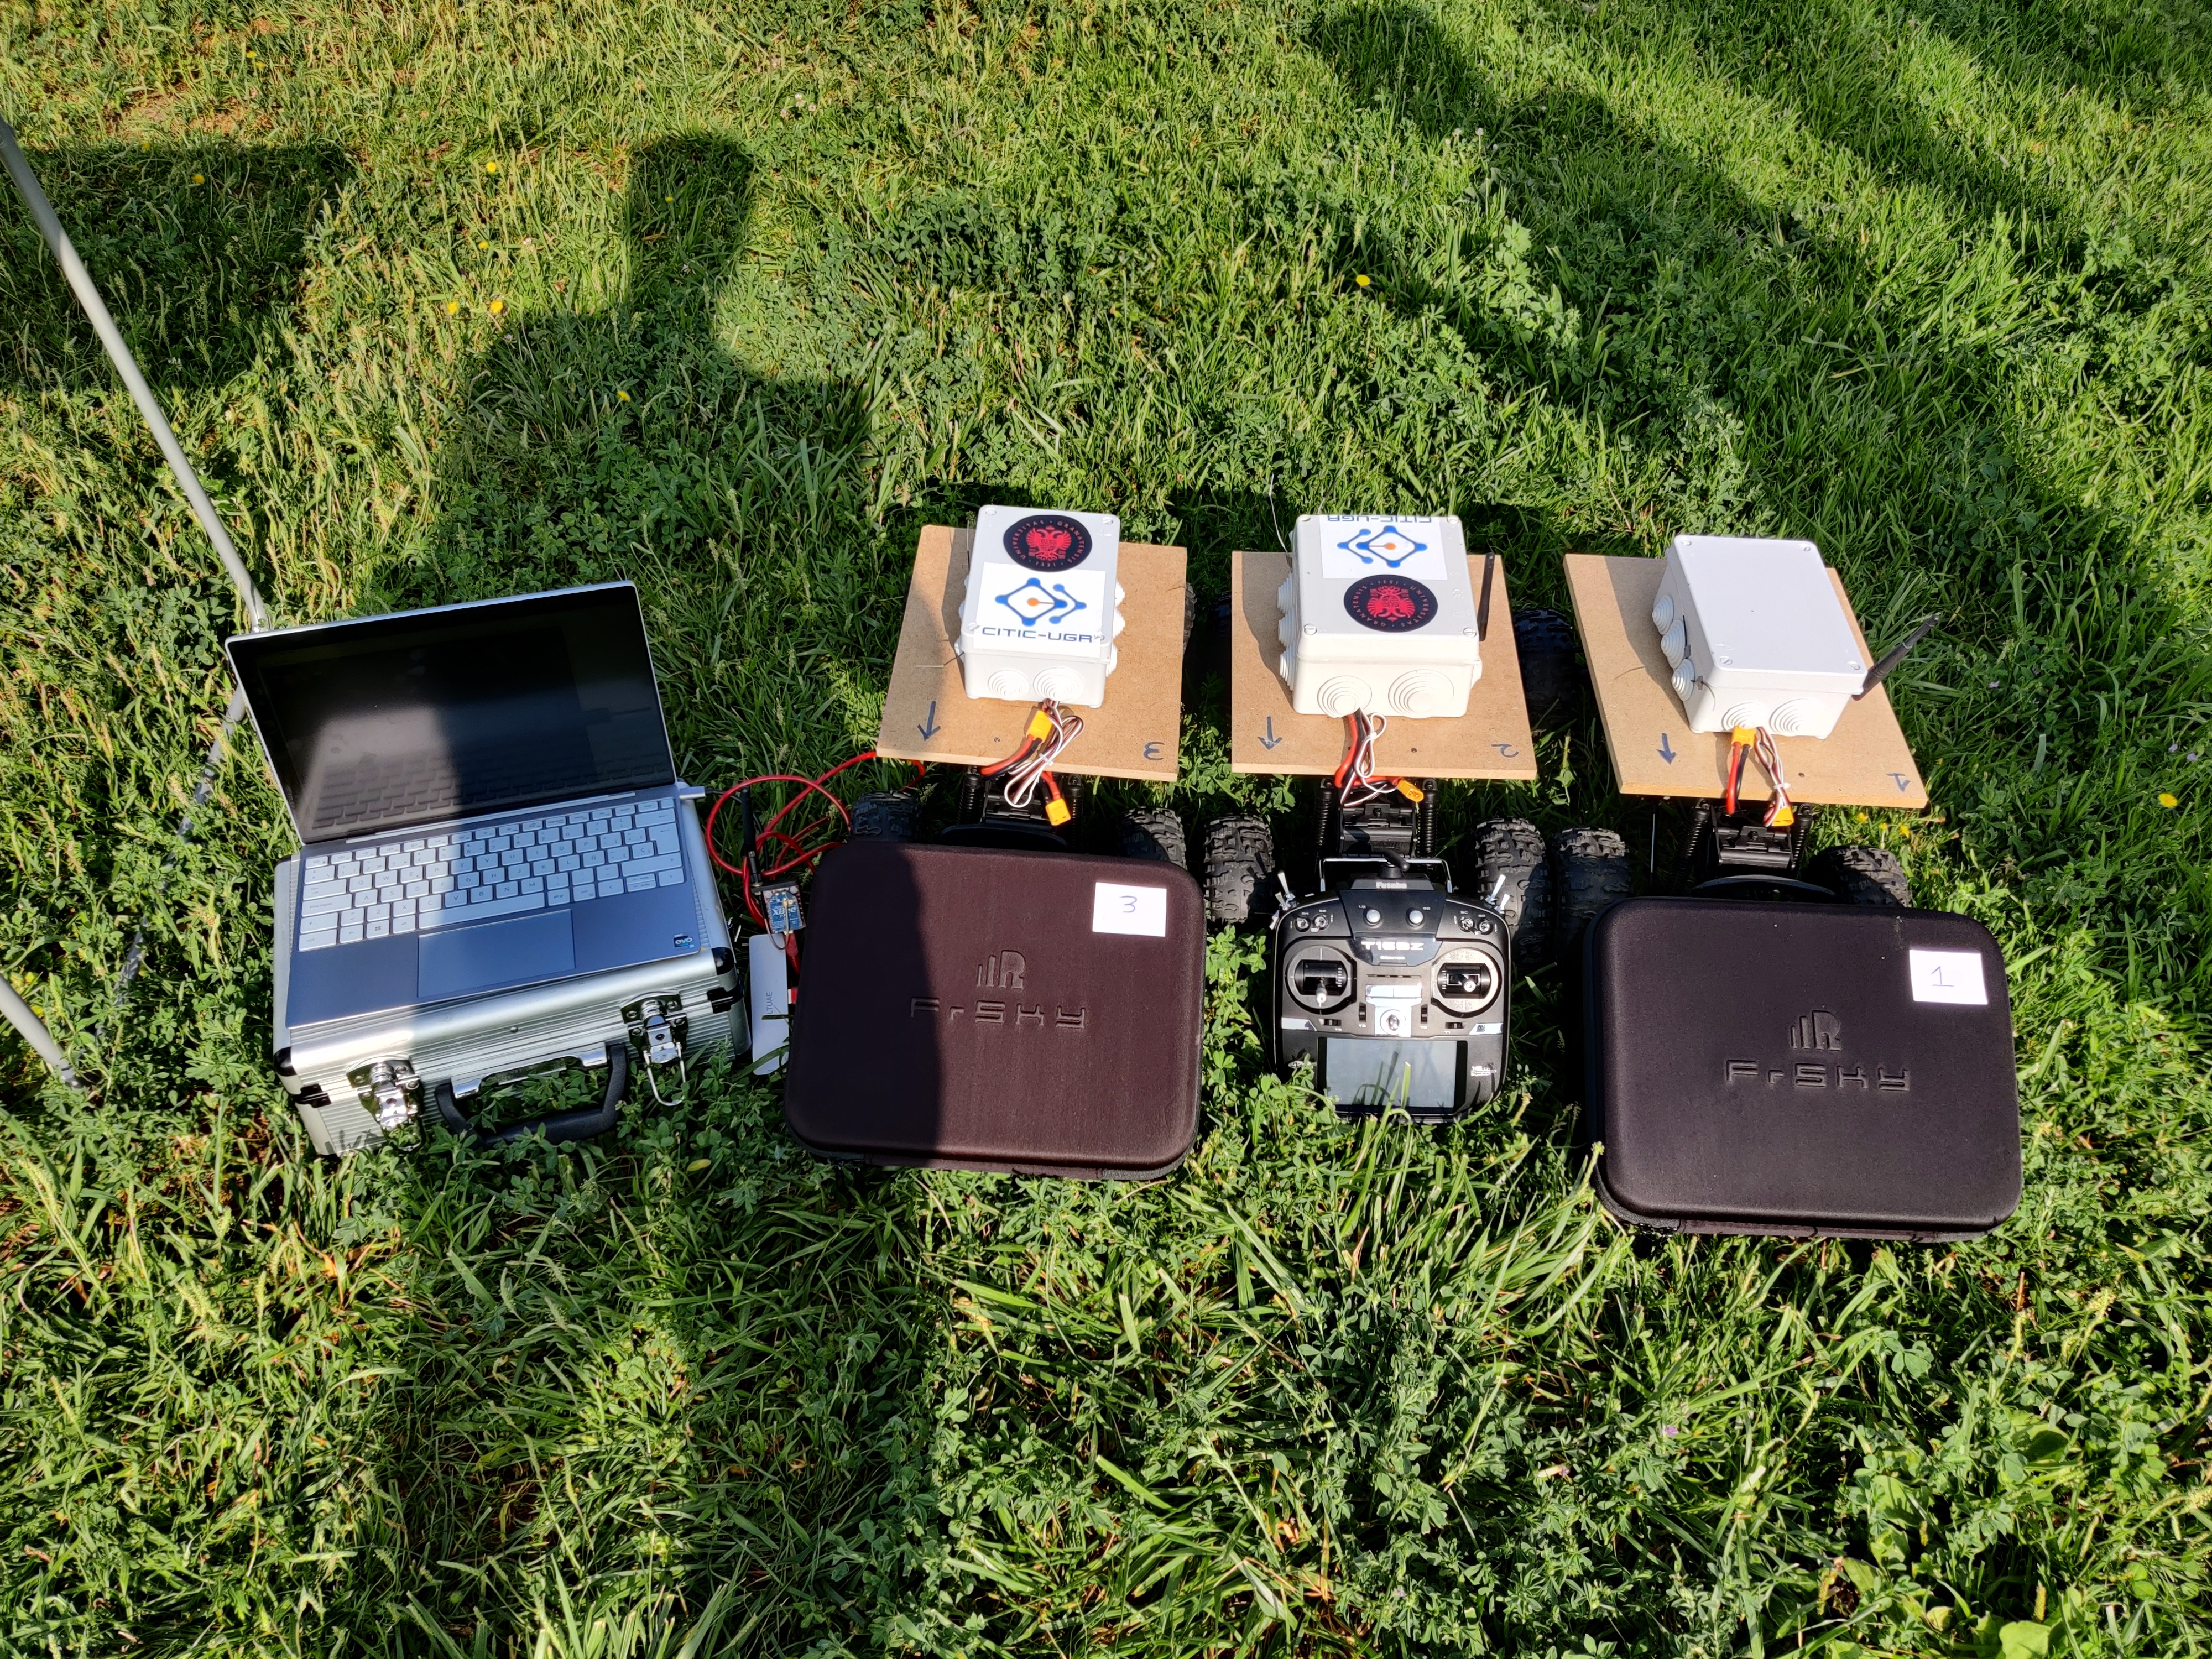
\includegraphics[trim={0 -1cm 0 0cm}, clip, width=1\textwidth]{fig/IMG_1.jpg}
    \caption{En esta imagen se muestra a la flota completa de \textit{rover}. A la izquierda tenemos la estación de tierra (PC + radio XBee) y a la derecha los tres \textit{rovers}, junto a sus emisoras de radio control.}
    \label{fig: rover_fleet}
\end{figure}

\newpage

\begin{figure}[h!]
    \centering
    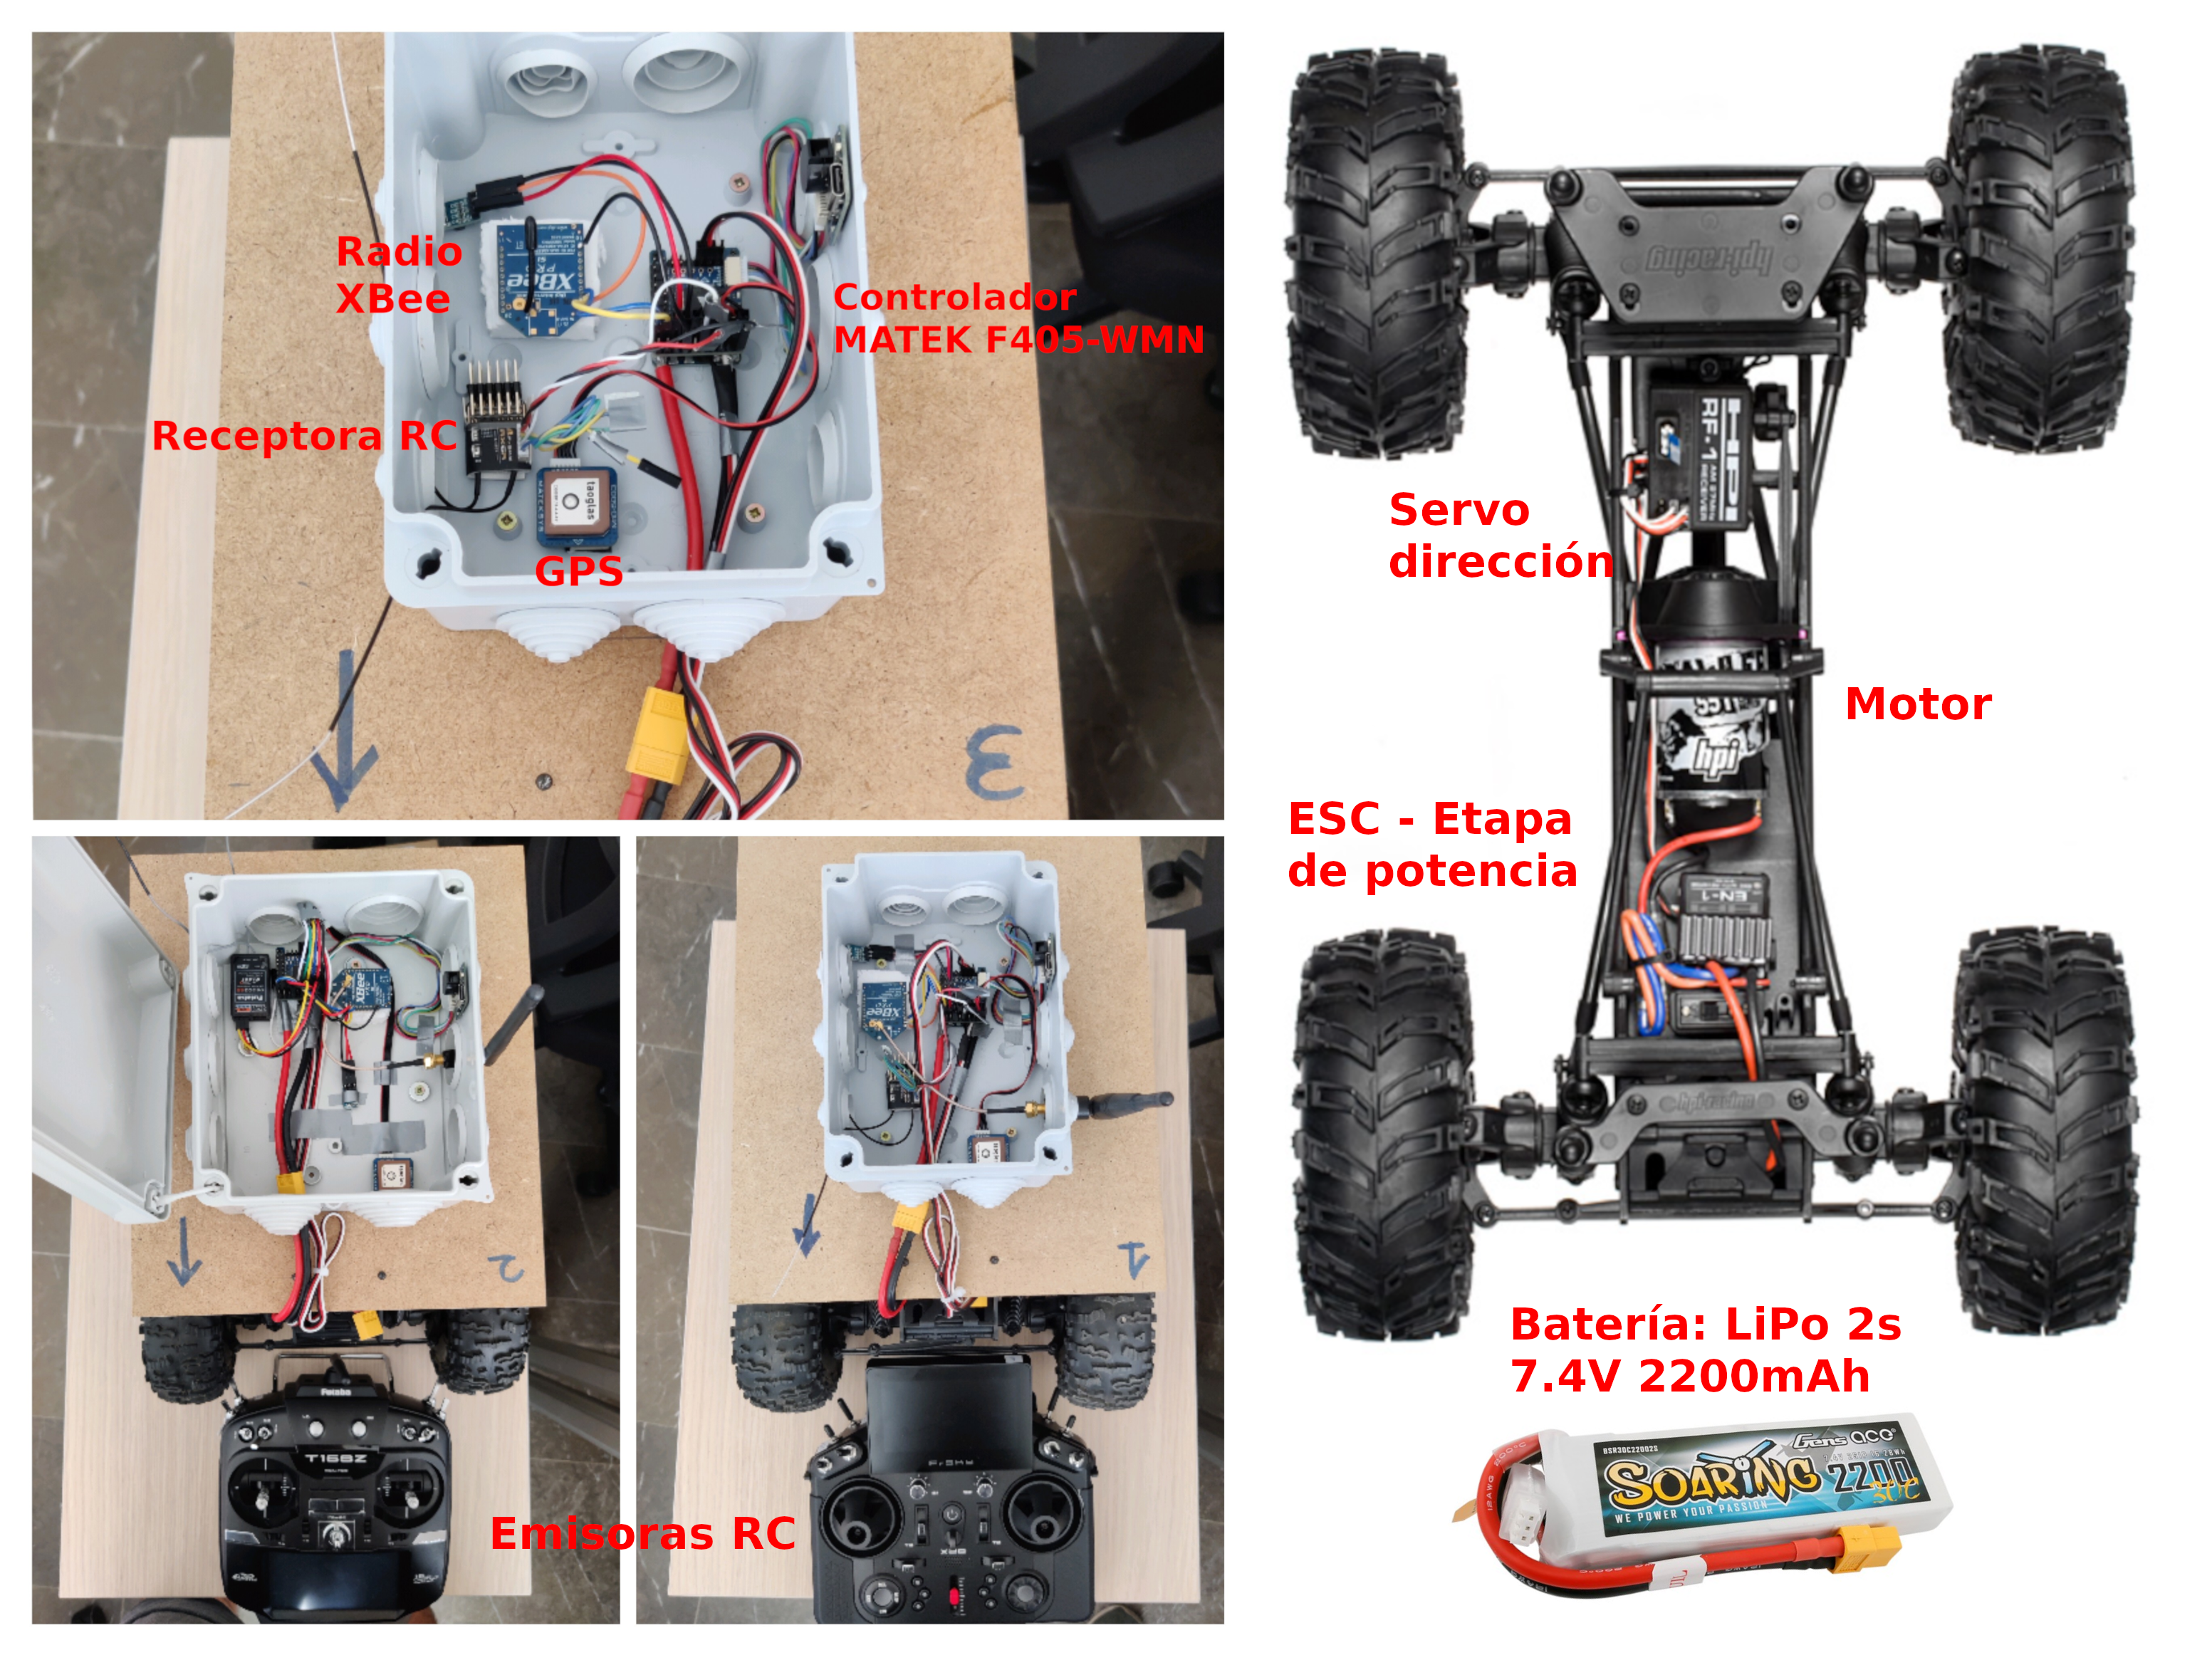
\includegraphics[trim={0 0cm 0 -1cm}, clip, width=0.9\textwidth]{fig/rover_elect.png}
    \caption{En esta figura se muestra la electrónica de todos los \textit{roves}. A la izquerda, tenemos el contenido de la caja estanca, mientras que a la derecha se pueden visualizar todos los componentes de chasis. Cada uno de estos \textit{rover} consta de un controlador principal al que se conecta el variador del motor, repectora RC, GPS, radio, servo de dirección y, por supuesto, batería.}
    \label{fig: rover_elct}
\end{figure}

\subsubsection{Integración distribuida del algoritmo de seguimiento de caminos y resultados}

Todo el software de los robots se ha desarrollado dentro del marco de Paparazzi UAS \cite{paparazzi}, un proyecto de hardware y software libre que cuenta con gran cantidad de drivers y herramientas para programar y trabajar con robots no tripulados.

Trabajar dentro de este entorno nos facilitó enormemente la tarea de integrar todos los subsistemas de cada \textit{rover}. No obstante, el proyecto no disponía de drivers para el controlador (Matek F405 WMN) y la IMU (ICM 42688-P) que nosotros habíamos seleccionado, por lo que el autor de este TFM se encargó de desarrollarlos. Además de estos driver, el autor también contribuyo a mejorar la estación de tierra implementando una herramienta para visualizar los campos vectoriales de guiado \cite{pull_gcs} y diseñó los sistemas de guiado y navegación para rovers con volante \cite{pull_sr}.

El controlador CBF se ha integrado en los robots de forma completamente distribuida. Es decir, son los propios robots los que se encargar de compartir entre ellos toda la información necesaria, haciendo uso de sus radios. La estación de tierra (ver \autoref{fig: rover_fleet}) únicamente se utiliza para visualizar la telemetría y mandar ordenes a los robots, por lo que no es fundamental para que el enjambre pueda llevar a cabo su misión de forma autónoma.

\newpage

En las Figuras \ref{fig: exp1}, \ref{fig: exp2} y \ref{fig: exp3} se pueden visualizar los instantes más relevantes de la prueba de campo realizada con la flota de \textit{rover}. En este experimento, a todos los robots se les ha indicado que sigan el mismo camino elíptico en sentido horario. Una vez que todos los robots se encuentren en modo asistido, el ángulo de giro de las ruedas vendrá modulado automáticamente por el controlador de a bordo, mientras que la celeridad será controlada manualmente desde una emisora RC. Téngase en cuenta que, en este modo asistido, tanto el controlador GVF (con $k_e$ = $k_d$ = 1) como el CBF (con $r$ = 2 y $\gamma$ = 0.4) se encontrarán activos. 

Por regla general, en la telemetría recogida por la estación de tierra podemos observar un comportamiento muy similar al de las simulaciones numéricas. El controlador CBF logra mantener a los \textit{rovers} fuera de la zona de colisión siempre que la acción de control $u_{safe}$ exigida es alcanzable. No obstante, en la realidad hay que tener muy en cuenta la precisión y desviación del GPS, pues no todos los robots tienen por qué estar donde realmente dicen estar. Dada una medida GPS, siempre se tiene que tener en cuenta un radio de incertidumbre de entorno a 1 o 2 metros. Es por esta razón, que al controlador CBF le indicamos un radio de colisión de 2 metros, para intentar lidiar con la imperfección inherente en la medida GPS. No obstante, a pesar de tomar esta precaución, la imprecisión de las medidas reales nos sigue pudiendo llevar a situaciones en las que, aunque la telemetría nos diga que todo va bien, los \textit{rovers} hayan colisionado. Esto es precisamente lo que sucede en el último instante de la \autoref{fig: exp3}, donde \textit{rover} 3 ha colisionado en la realidad con el 1 al intentar esquivarlo.

Resulta muy interesante fijarse especialmente en el instante t = 287 de la \autoref{fig: exp1}, donde el \textit{rover} 2, que se encuentra esquivando al 1, tiene que adaptarse rápidamente para evitar colisionar con el \textit{rover} 3, pues éste ha decidido realizar un giro muy brusco para esquivar al \textit{rover} 1. Es es un caso muy bonito, pues además de verificar experimentalmente el Teorema \ref{thm: cbf} y la Proposición \ref{prop: multi_cbf}, también permite ilustrar la robustez de nuestro algoritmo ante casos extremos.

\vspace{1cm}

\begin{figure}[h!]
    \centering
    \includegraphics[trim={0 0cm 3.8cm 0cm}, clip, width=0.48\textwidth]{fig/231.png}
    \includegraphics[trim={0 0cm 0 0cm}, clip, width=0.48\textwidth]{fig/data_231.png}
    \caption{En esta figura se visualizan los resultados del experimento entre t = 201 y t = 231. En este intervalo de tiempo, el \textit{rover} 3 se encuentra adelantando al 1 y 2, que se encuentran parados. A la izquierda se visualiza el camino a seguir y la trazada los robots, mientras que en los gráficos de la derecha se visualizan todos los $\psi_{ij}$ y la acción de control $u_{safe}^i$ que actúa sobre cada robot.}
    \label{fig: exp1}
\end{figure}

\begin{figure}[h!]
    \centering
    \includegraphics[trim={0 0cm 0 0cm}, clip, width=0.48\textwidth]{fig/297.png}
    \includegraphics[trim={0 0cm 0 0cm}, clip, width=0.48\textwidth]{fig/data_297.png}
    \caption{En esta figura se visualizan los resultados del experimento entre t = 297 y t = 257. En este intervalo de tiempo, el \textit{rover} 2 se encuentra adelantando al 1 y 3, al mismo tiempo que el \textit{rover} 3 adelanta al 1, que se entra parado. Véase que el \textit{rover} 2 tiene que hacer un giro bastante brusco en t = 288 para esquivar al \textit{rover} 3. A la izquierda se visualiza el camino a seguir y la trazada los robots, mientras que en los gráficos de la derecha se visualizan todos los $\psi_{ij}$ y la acción de control $u_{safe}^i$ que actúa sobre cada robot.}
    \label{fig: exp2}
\end{figure}

\newpage

\begin{figure}[h!]
    \centering
    \includegraphics[trim={0 0cm 0 0cm}, clip, width=0.48\textwidth]{fig/358.png}
    \includegraphics[trim={0 0cm 0 0cm}, clip, width=0.48\textwidth]{fig/data_358.png}
    \caption{En esta figura se visualizan los resultados del experimento entre t = 358 y t = 318. En este intervalo de tiempo, el \textit{rover} 2 se encuentra adelantando al 1 y 3, al mismo tiempo que el \textit{rover} 3 adelanta al 1, que se entra parado. A la izquierda se visualiza el camino a seguir y la trazada los robots, mientras que en los gráficos de la derecha se visualizan todos los $\psi_{ij}$ y la acción de control $u_{safe}^i$ que actúa sobre cada robot.}
    \label{fig: exp3}
\end{figure}

%%%%%%%%%%%%%%
% Conclusión %
%%%%%%%%%%%%%%

\vspace{-0.3cm}
\subsection{Conclusiones}

A lo largo de esta metodología, hemos presentado una serie de resultados originales que permiten resolver de forma robusta y efectiva el problema de garantizar la ausencia de colisiones en el seguimiento de caminos con enjambres robóticos. Además de verificar numéricamente todos estos resultados teóricos, se ha construido toda una flota de \textit{rover} que han permitido verificar experimentalmente la viabilidad práctica de nuestro algoritmo.

De cara a un trabajo futuro, se podría pensar en tratar de generalizar nuestros resultados lo máximo posible, intentando deshacernos de todas las suposiciones que limitan las capacidades prácticas de nuestro algoritmo. Si se lograra alcanzar este punto, estaríamos hablando de una solución completamente novedosa y con una enorme cantidad de aplicaciones reales.